%% Déclare un article sur feuille A4
\documentclass[a4paper]{article}

%% Langues et encodages des polices d'écriture
\usepackage[frenchb]{babel}
\usepackage[utf8]{inputenc}
\usepackage[T1]{fontenc}

%%  Choisis la page et les marges 
\usepackage[a4paper,top=3cm,left=3cm,right=3cm,headsep=45pt,marginparwidth=1.75cm]{geometry}

%% Importe les packages dont on a besoin dans le rapport
\usepackage{lastpage}
\usepackage{graphicx}
\usepackage{caption}
\usepackage[colorlinks=true, allcolors=blue]{hyperref}

\usepackage{float}
\usepackage{fancyhdr}

\fancyhf{}
\lhead{
    
\includegraphics[scale=0.25]{img/logobyes.png}
    
\includegraphics[scale=0.17]{img/logo-bouygues-construction.jpg}
}
\rhead{
    
\includegraphics[scale=0.1]{img/logo-univ.png}
    
\includegraphics[scale=0.0425]{img/logo-iut.png}
    
\includegraphics[scale=0.31]{img/logo-info.png}
}
\renewcommand{\footrulewidth}{0.4pt}
\fancyfoot{
    Pinon Olivier - IUT Annecy - Département Informatique - 2016/2017
    \hfill
    \thepage{} / \pageref*{LastPage}
}


\begin{document}

    \pagestyle{fancy}
    \thispagestyle{empty}
    \noindent
    \begin{minipage}{.5\textwidth}
        Bouygues Energies et Services \\
        49 avenue du Lac du Bourget \\
        73375 Le Bourget du Lac, France
    \end{minipage}
    \begin{minipage}{.5\textwidth}
    \begin{flushright}
        Pinon Olivier \\
        IUT d'Annecy \\
        DUT INFO \\
        Année 2016/2017 \\
    \end{flushright}
    \end{minipage}
    
    \vfill 
    \begin{center}
		\Huge{\textbf{Rapport de stage : }} \\
        \vspace{20pt}
        \Large{Développement d'un module d'habilitation éléctrique en réalité virtuelle sur moteur de jeu Unity}
        
	\end{center}
    \vfill 
    
    Palanca Jérôme  \hfill Damas Luc

 	\newpage 
     % Remerciements 
    \huge \textbf{Remerciements} \vspace{10pt} \\

    \normalsize
    Je souhaite tout d'abord remercier Monsieur Jérôme PALANCA, mon tuteur de stage, pour la confiance, l'écoute et la sympathie dont il a fait preuve à mon égard. Il a su m'aider à comprendre les problèmes de nature inconnue qui m'étaient posés et a su accepter mes propositions tout en me proposant des améliorations. Le suivi quotidien qu'il a effectué m'a permis de constamment garder en tête les objectifs et ainsi de me guider pas à pas dans le projet. \vspace{10pt} \\

    J'adresse aussi mes remerciements à Monsieur Renaud PAYERNE, qui est à l'origine du projet peu commun sur lequel j'ai travaillé, et m'a permis d'obtenir le stage. \vspace{10pt} \\
	Merci également à Monsieur Luc DAMAS, pour son suivi en cours de stage qui m'a donné de précieuses indications sur le contenu et les axes à souligner dans mon rapport et ma soutenance. \vspace{10pt} \\

    Finalement, je tiens à remercier l'ensemble du bureau d'études de Bouygues Energies et Services. Merci à cette équipe qui a su m'accueillir malgré nos travaux très différents, et qui m'a fait passé un très bon stage dans la bonne humeur quotidienne du bureau. Ils ont su me donner un aperçu du monde du travail très plaisant, à la fois sérieux dans les heures de travail, et détendu dans les moments de pause. \vspace{10pt} \\

    Grâce à leur confiance, à leurs réponses et à leur avenance, j'ai pu apprendre beaucoup sur le monde professionnel. Travailler à leur côtés a été un véritable plaisir, et une experience très enrichissante. \\
    
    \newpage
    % Table des matières 
    \setcounter{tocdepth}{2}
    \tableofcontents

    \newpage 
    % Introduction 
    \huge \textbf{Introduction} \vspace{20pt} \\
    \normalsize
    Afin de finaliser mon diplôme de DUT Informatique à l'IUT d'Annecy, j'ai effectué mon stage d'une durée de 3 mois dans une entreprise de mon choix, qui s'est naturellement porté vers le secteur de l'industrie, puisque je souhaite continuer mes études dans une école d'ingénieur industriel. \\

    Par l'intermédiaire de madame Nathalie Gruson, j'ai répondu à une annonce qui m'a particulièrement intéressé puisqu'elle proposait de travailler sur de la réalité virtuelle\footnote{La réalité virtuelle est une technique graphique visant à utiliser un casque projetant des images en 3D à un utilisateur afin d'améliorer l'immersion de celui-ci dans le monde qui l'entoure} en utilisant Unity, un moteur de jeu que j'ai l'habitude d'utiliser, et qui est une technologie que j'affectionne particulièrement. \\

    L'entreprise n'a rien à voir avec le secteur de l'informatique pure, et c'est justement cette différence avec les autres offres de stage qui m'a poussé à candidater, afin de découvrir un autre monde que les sites et applications web et mobiles, que l'on pratique beaucoup à l'IUT. \\
    
    Bouygues Energies et Services m'a proposé de travailler sur un nouveau module, qui permettrait d'aider leurs techniciens à se former à la maintenance de cellules dites HT (Haute Tension), en mettant à profit les nouvelles technologies, notamment la réalité virtuelle. \\

    Durant ce rapport, je ferais des explications à propos des technologies utilisées en restant le plus clair et simple possible. Pour plus d'informations techniques, j'ai écris une documentation technique d'une cinquantaine de pages sur mon projet. \\

    Dans la première partie, je présenterais l'entreprise qui m'a accueilli. Puis, je développerai le besoin et la mission que l'on m'a assigné. J'expliquerais ensuite la phase d'étude et de réalisation du projet, et je finirai par un bilan de l'experience enrichissante qu'a été ce stage. \\

    \newpage 
    % Présentation générale 
    \section{Présentation générale de l'entreprise}

    \subsection{Le groupe Bouygues et ses filiales}

    Bouygues est un groupe industriel diversifié français fondé en 1952 par Francis Bouygues et dirigé par son fils Martin Bouygues depuis 1989. \\

    Le groupe est structuré autour de trois activités : le secteur BTP (Bouygues Construction,
Bouygues Immobilier et Colas), les réseaux de télécommunication (Bouygues Telecom) et les médias (TF1). Chaque sous-groupe comprend des filales. Bouygues Energies et Services, par exemple, est une filiale du sous-groupe Bouygues Construction, lui même appartenant au groupe Bouygues. Il est à noter que Bouygues Energies et Services a été renommé en 2013 ; Il s'agissait auparavant de l'entreprise ETDE, rachetée par Bouygues Construction en 1984. \\

    \begin{figure}[H]
    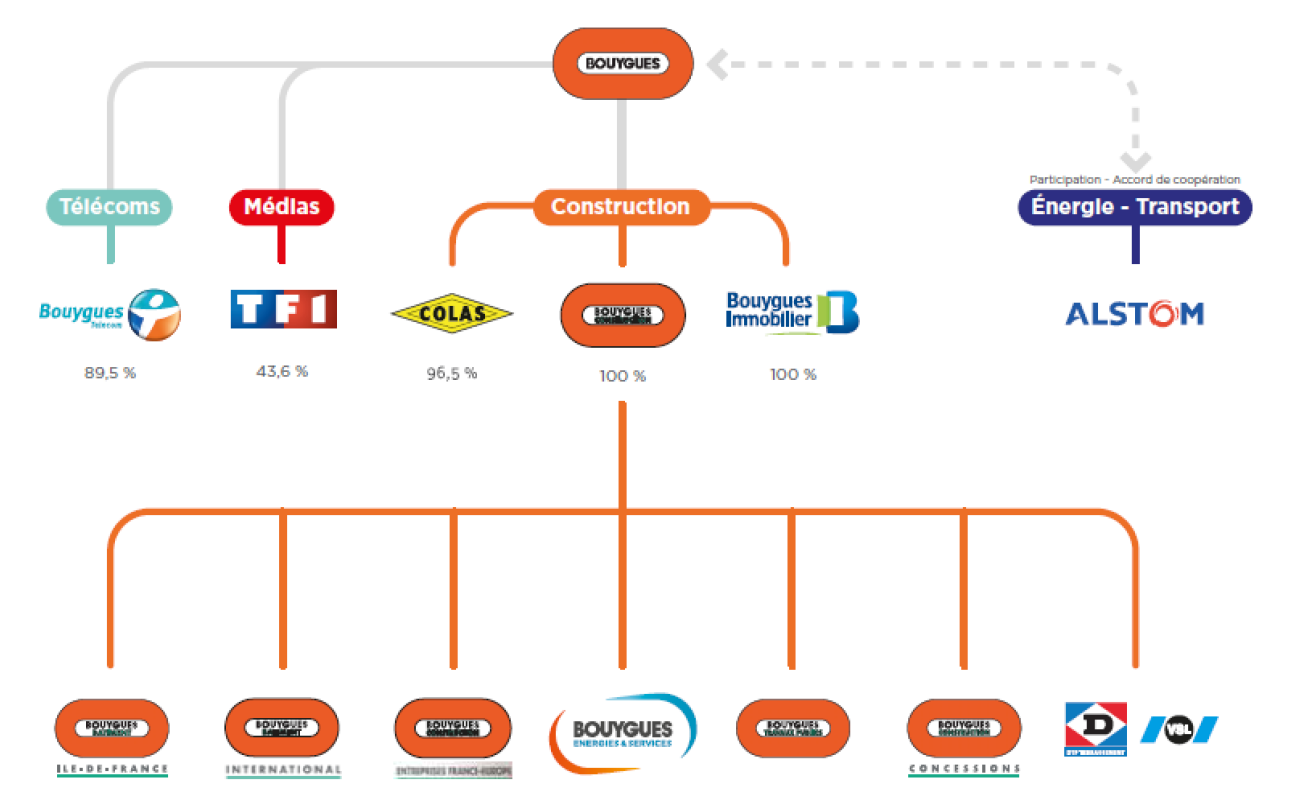
\includegraphics[scale=0.45]{img/groupeBouygues}
    \end{figure}

    Le groupe Bouygues est un des leaders du marché dans tous les secteurs où il possède des groupes. En 2015, le chiffre d’affaires du groupe Bouygues s’élève à 32,428 milliards d’euros, et celui de Bouygues Energies Services s'élève à 925 568 300 euros. \\

    \subsection{Produits et services}
 
    \subsubsection{L'activité de Bouygues Energies et Services}
    Bouygues Energies et Services est une filiale dont l'activité est découpée sur 4 marchés principaux : \\
    
    \begin{itemize}

    \item Les infrastructures numériques : \\
        
        Bouygues Energies et Services connecte les territoires afin que tous puissent bénéficier des avantages du tout numérique. Grâce à son savoir-faire et son expertise mises au service de la création et la modernisation des infrastructures de télécommunication et du numérique, l'entreprise relie et dynamise des territoires auparavant isolés. \\

    \item Les villes et collectivités : \\

        La population mondiale devenant de plus en plus urbaine, et le mouvement s'accélérant, la ville de demain doit être plus accueillante, économe, connectée et sécurisée, de façon à allier la qualité de vie avec une empreinte écologique faible\footnote{Mesure de la pression exercée par l'homme sur la nature}. Bouygues Energies et Services est un des acteurs de cette transition qui concerne les collectivités. \\

    \item Le tertiaire et l'industrie: \\

        Afin de les aider à accroître leur compétitivité, ou à optimiser leurs facture énergétique, Bouygues Energies et Services propose des solutions globales aux entreprise industrielles, dans le but de permettre d'améliorer les process mis en place. \\

    \item L'énergie et le transport : \\

        L'entreprise travaille en collaboration avec de grands clients et services publics, en proposant de nouvelles solutions techniques permettant de réduire les consommations et d'augmenter la qualité de nos transports et éclairages. 

    \end{itemize}
    \vspace{5pt}
    
    Le rôle des techniciens de Bouygues Energies et Services est de travailler en collaboration avec d’autres bureaux d’étude dont les spécialités sont le génie climatique et l’architecture, afin de concevoir le bâtiment et ses fonctionnalités avant d’envoyer les plans et de le construire sur le terrain. Fréquemment (presque toutes les semaines), les ingénieurs et chefs de projets sont amenés à se déplacer sur le terrain pour faire un point sur l’avancée des travaux, et discuter de l'implémentation des nouvelles solutions techniques envisagées par les bureaux d'étude. \\
 
    \subsubsection{Les grands projets de l'entreprise}

    Comme expliqué précédemment, l'entreprise travaille sur des grands projets du secteur public. Le domaine d'expertise de Bouygues Energies et Services est l'éléctricité, et notamment les problématiques existantes autour du stockage et du transport d'énergie avec des pertes toujours plus faibles. \\

    Dans le bureau d'étude dans lequel j'ai travaillé, les techniciens et ingénieurs sont en train d'étudier et de mettre en place de nouvelles solutions techniques sur des projets réels comme les stations de métro de Lyon (Lignes 1 et 2), l’autoroute A9 vers Montpellier, ou encore la nouvelle université de Marseille. \\

    \subsection{Implantation et locaux}
    \subsubsection{Bouygues Energies et Services en France et dans le monde}

    Le groupe Bouygues est présent dans plus de 100 pays sur les 5 continents. La société Bouygues Energies et Services, quant à elle, est implantée dans 25 pays d’Europe, d’Afrique et d’Amérique du Nord, suivant 7 zones géographiques (France IDF, France Ouest, France Est/Italie, Royaume Uni, Suisse/Allemagne, Canada, Afrique). Comptant près de 200 implantations sur le territoire Français, dont 35 dans notre zone (France Est/Italie), l’entreprise est donc 
    établie assez largement et dans le monde

    \begin{figure}[H]
    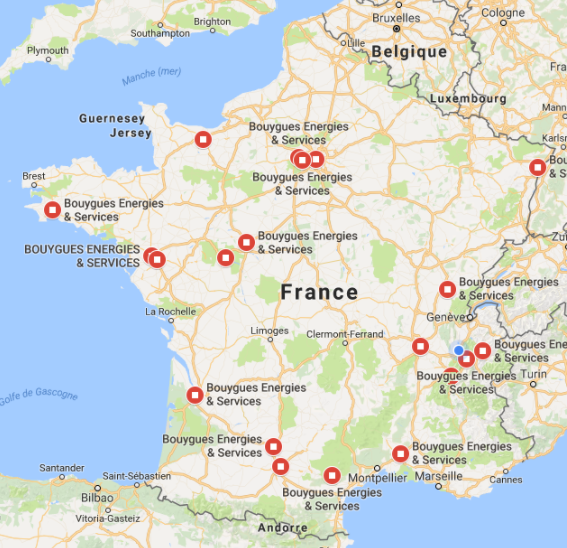
\includegraphics[scale=0.5]{img/implantationFrance}
    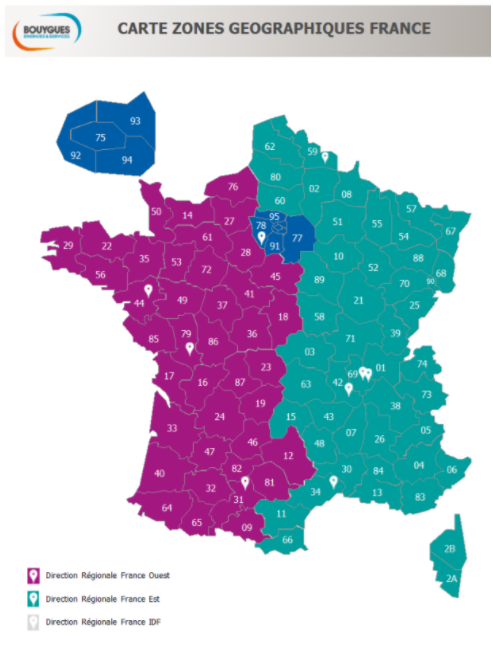
\includegraphics[scale=0.5]{img/ZGFrance}
    \caption{Implantation de Bouygues Energies et Services en France selon les zones géographiques}
    \end{figure}

    \subsubsection{Les locaux de l'entreprise}

    Dans le cadre de mon stage, j’ai travaillé dans les locaux du technopôle Savoie Technolac, plus précisément dans l'un des bureaux d’étude. \\

    \begin{figure}[H]
        \centering
        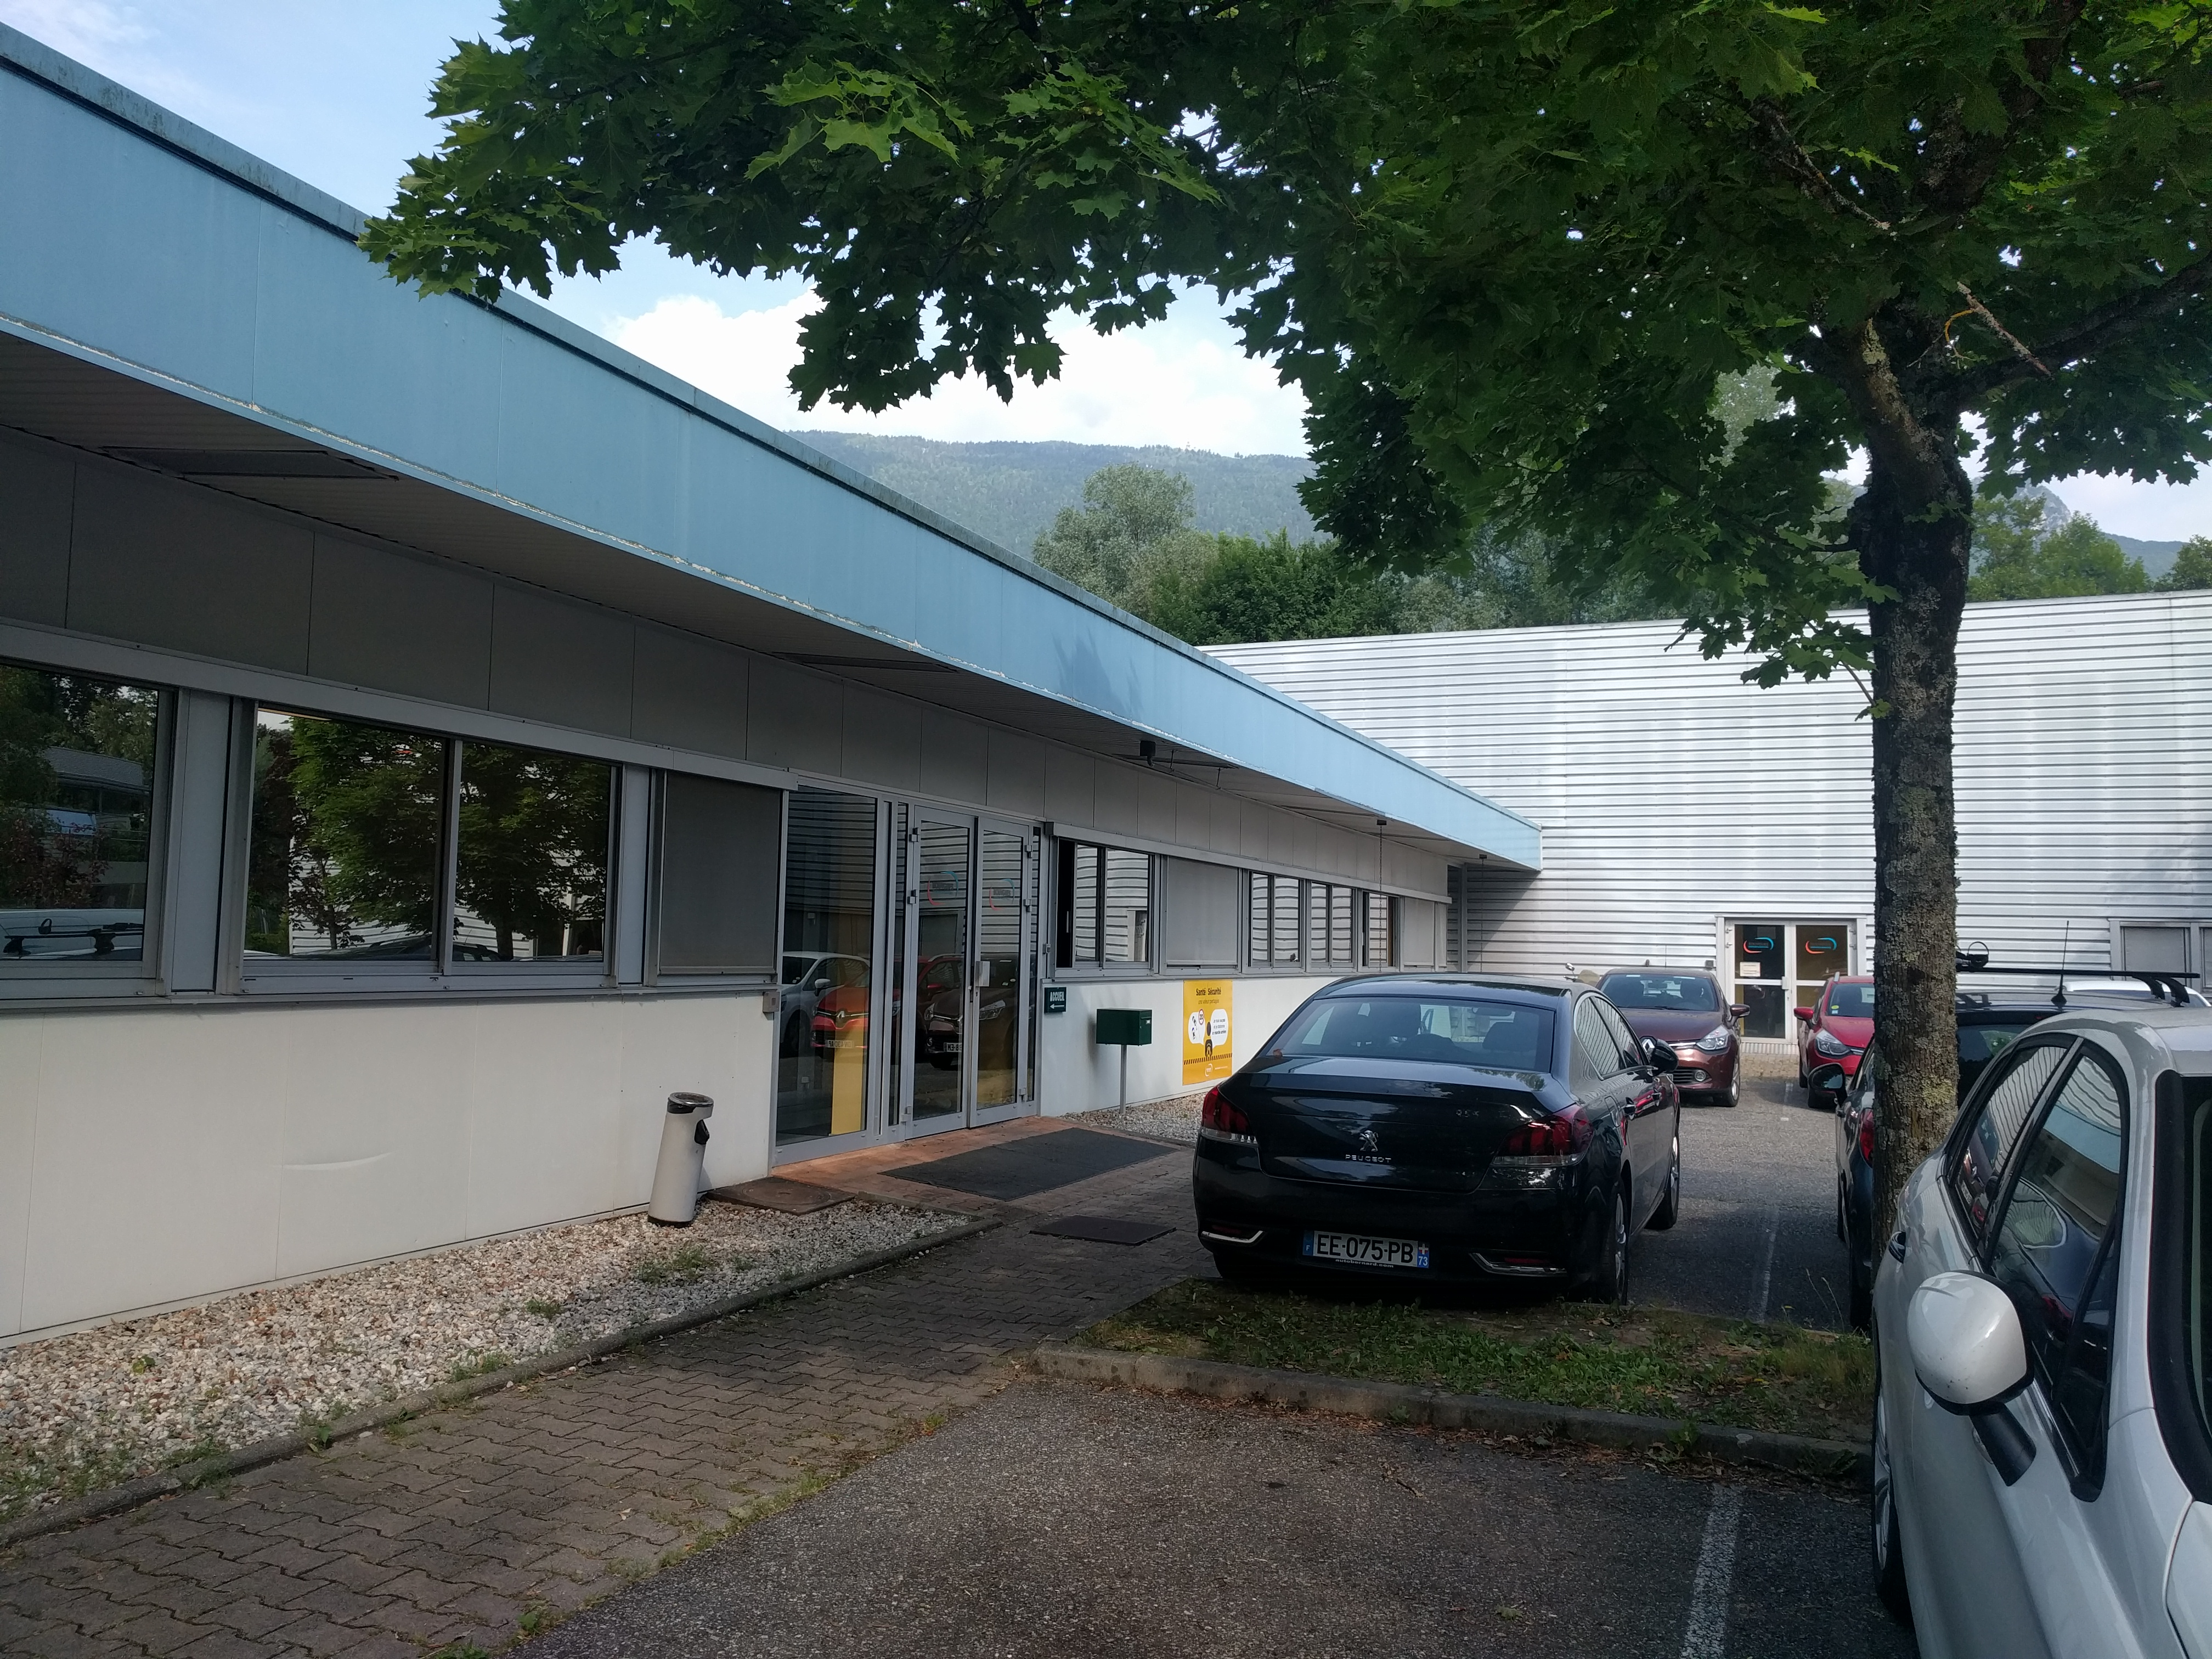
\includegraphics[scale=0.065]{img/imgLocaux}
        \caption{Les locaux de mon entreprise, vus de l'exterieur}
    \end{figure}
    \begin{figure}[H]
        \centering
        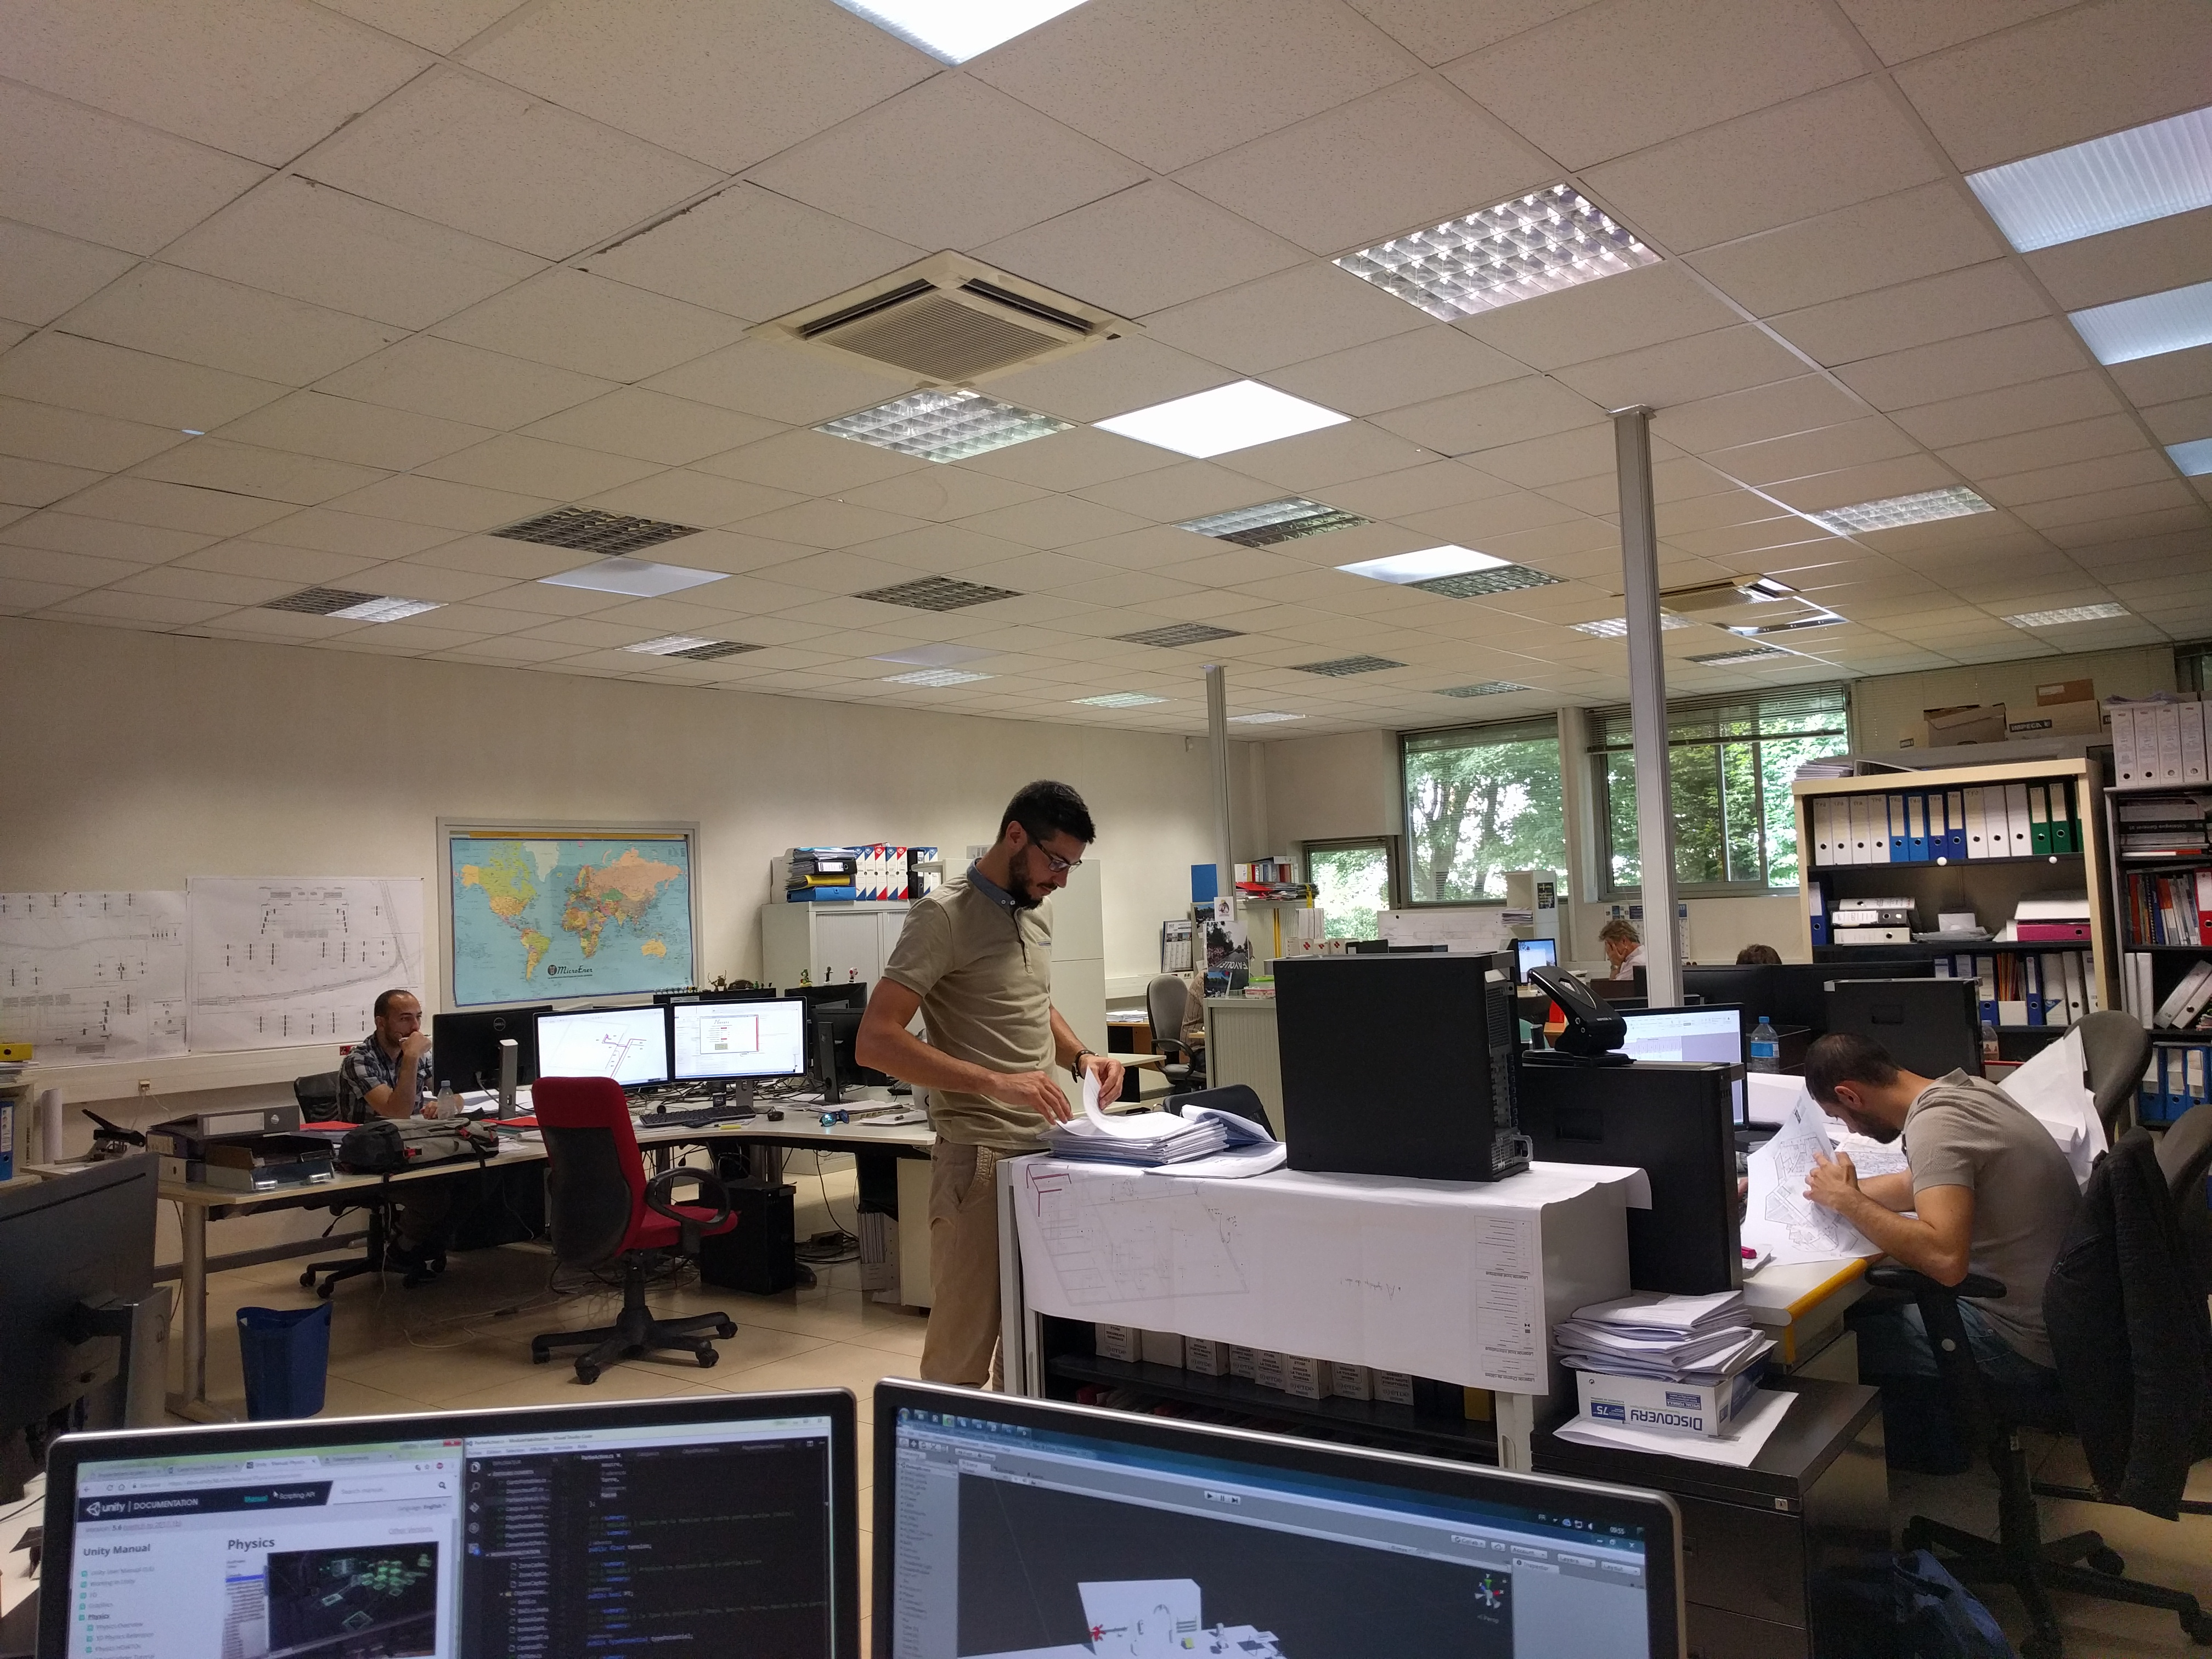
\includegraphics[scale=0.065]{img/bureauEtude}
        \caption{Le bureau dans lequel j'ai travaillé}
    \end{figure}
    \begin{figure}[H]
        \centering
        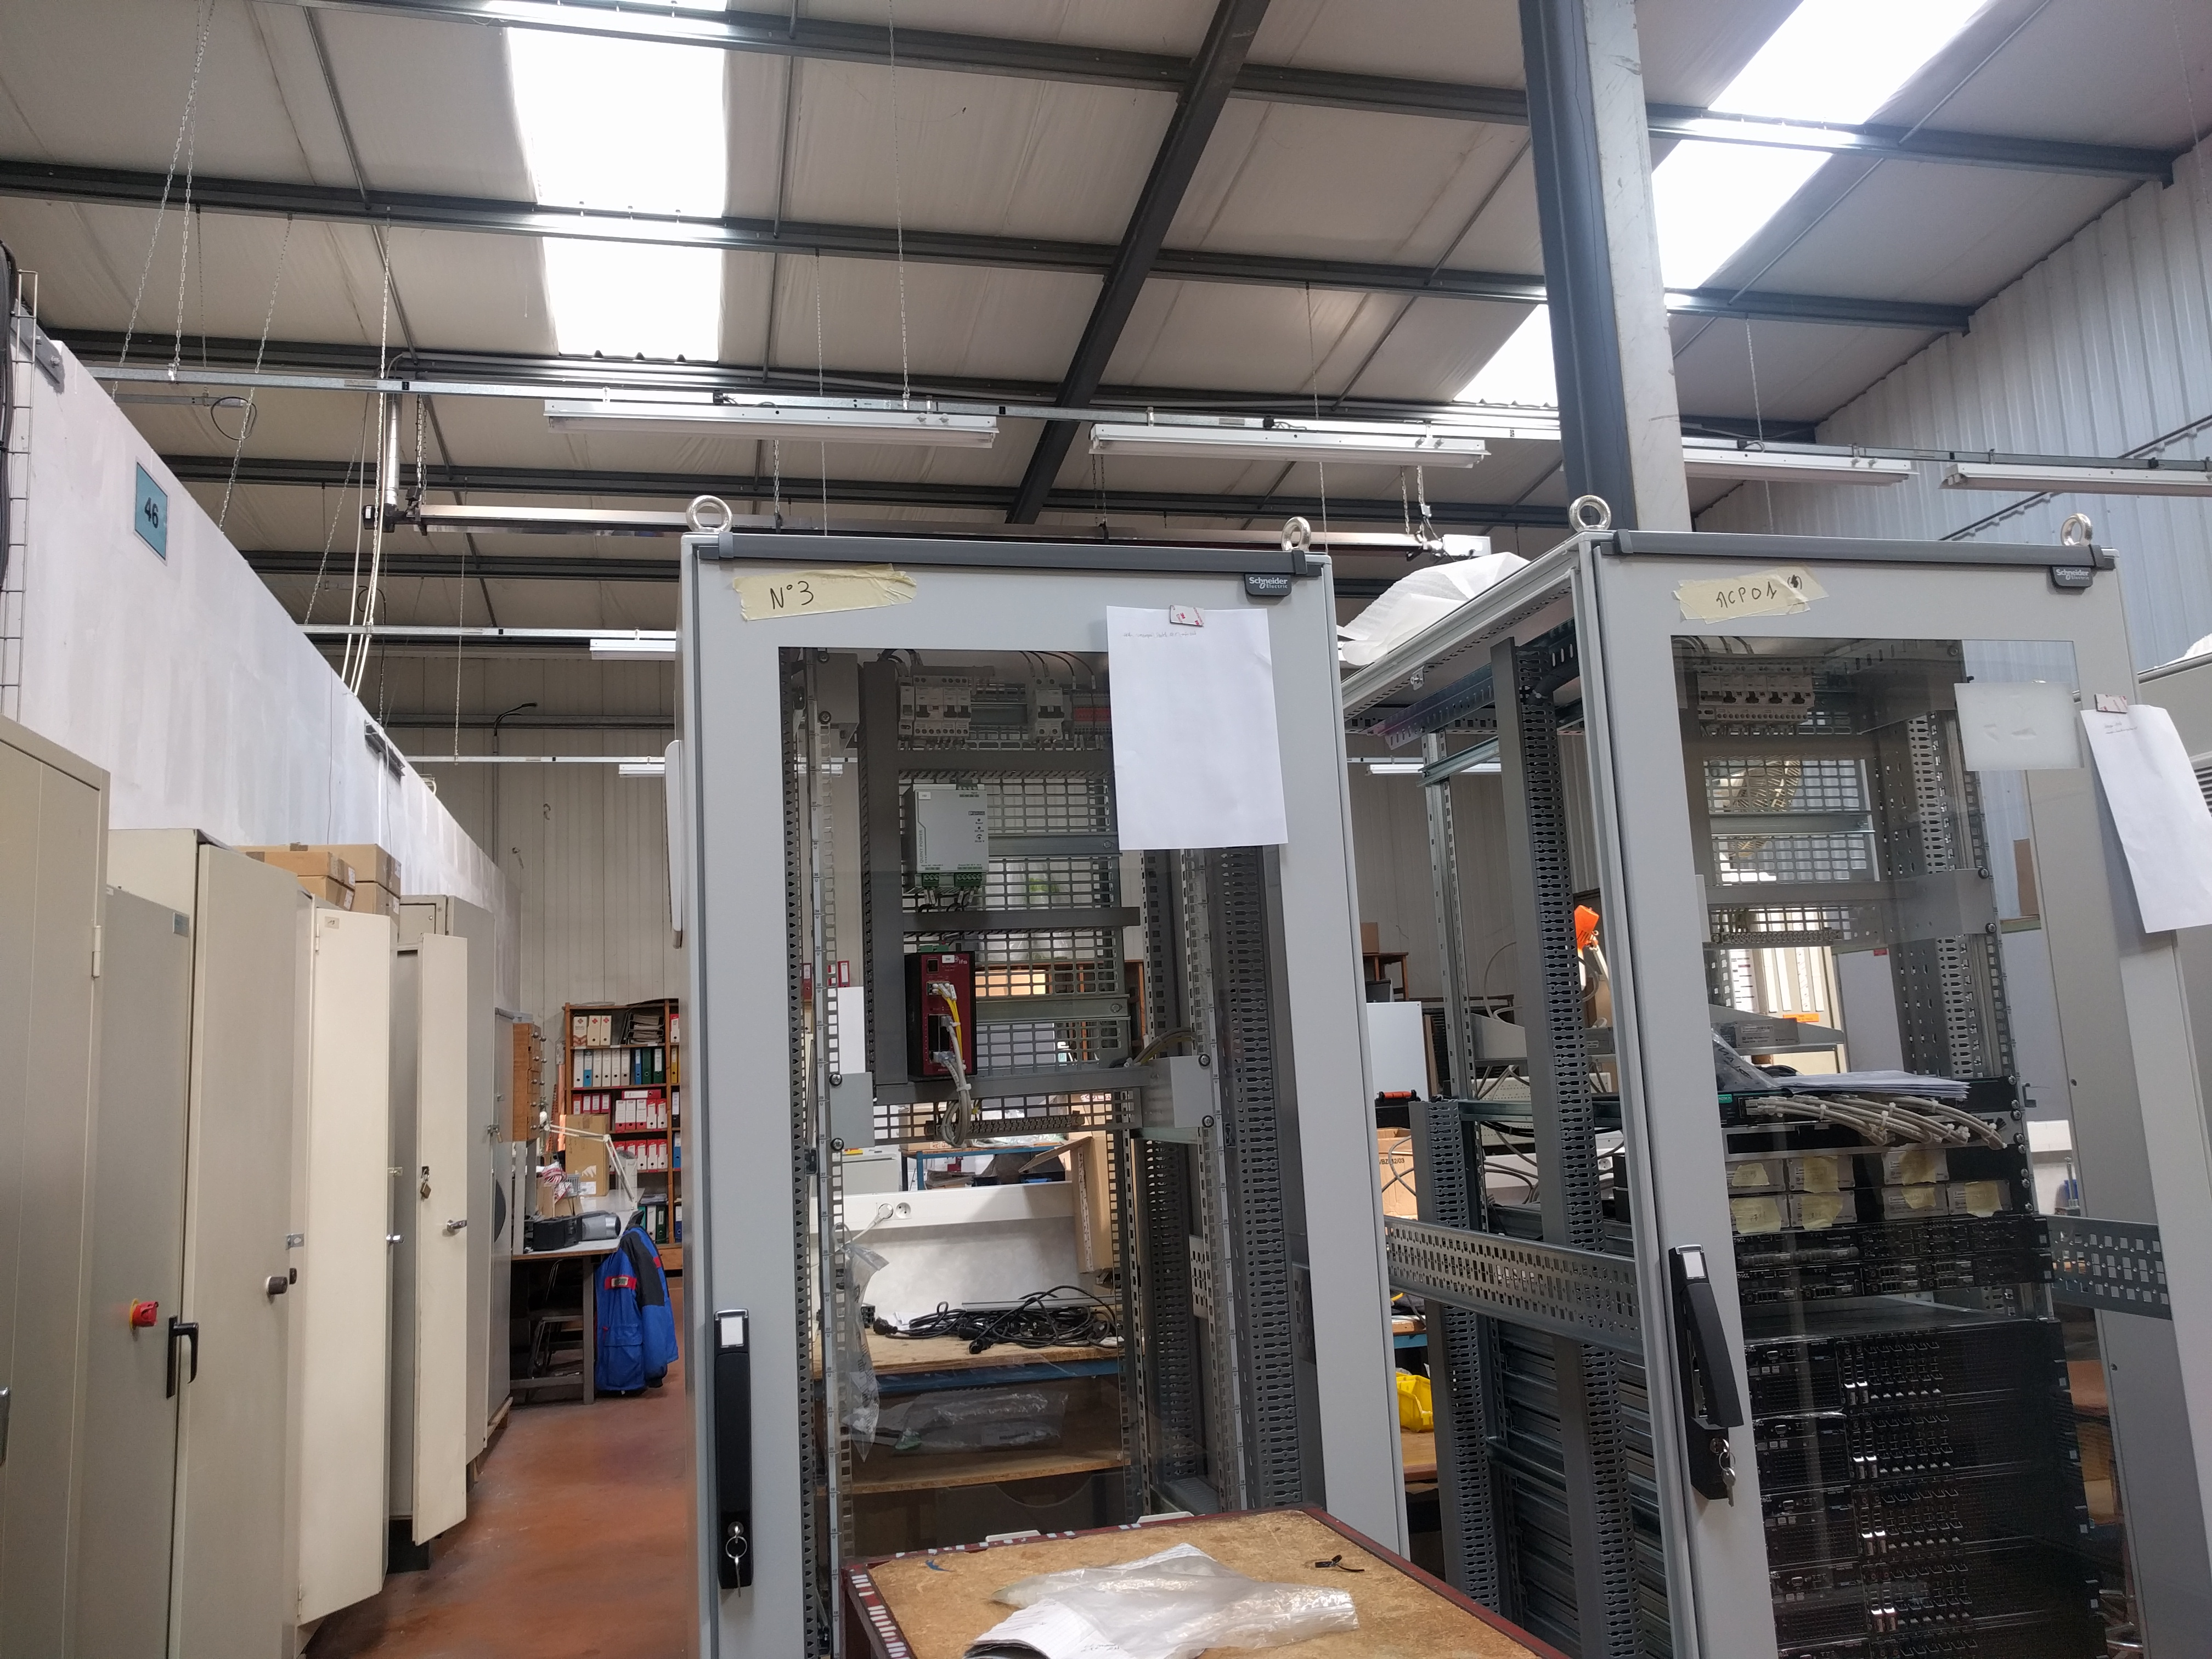
\includegraphics[scale=0.065]{img/atelier}
        \caption{L'atelier des électriciens}
    \end{figure}
    \begin{figure}[H]
        \centering
        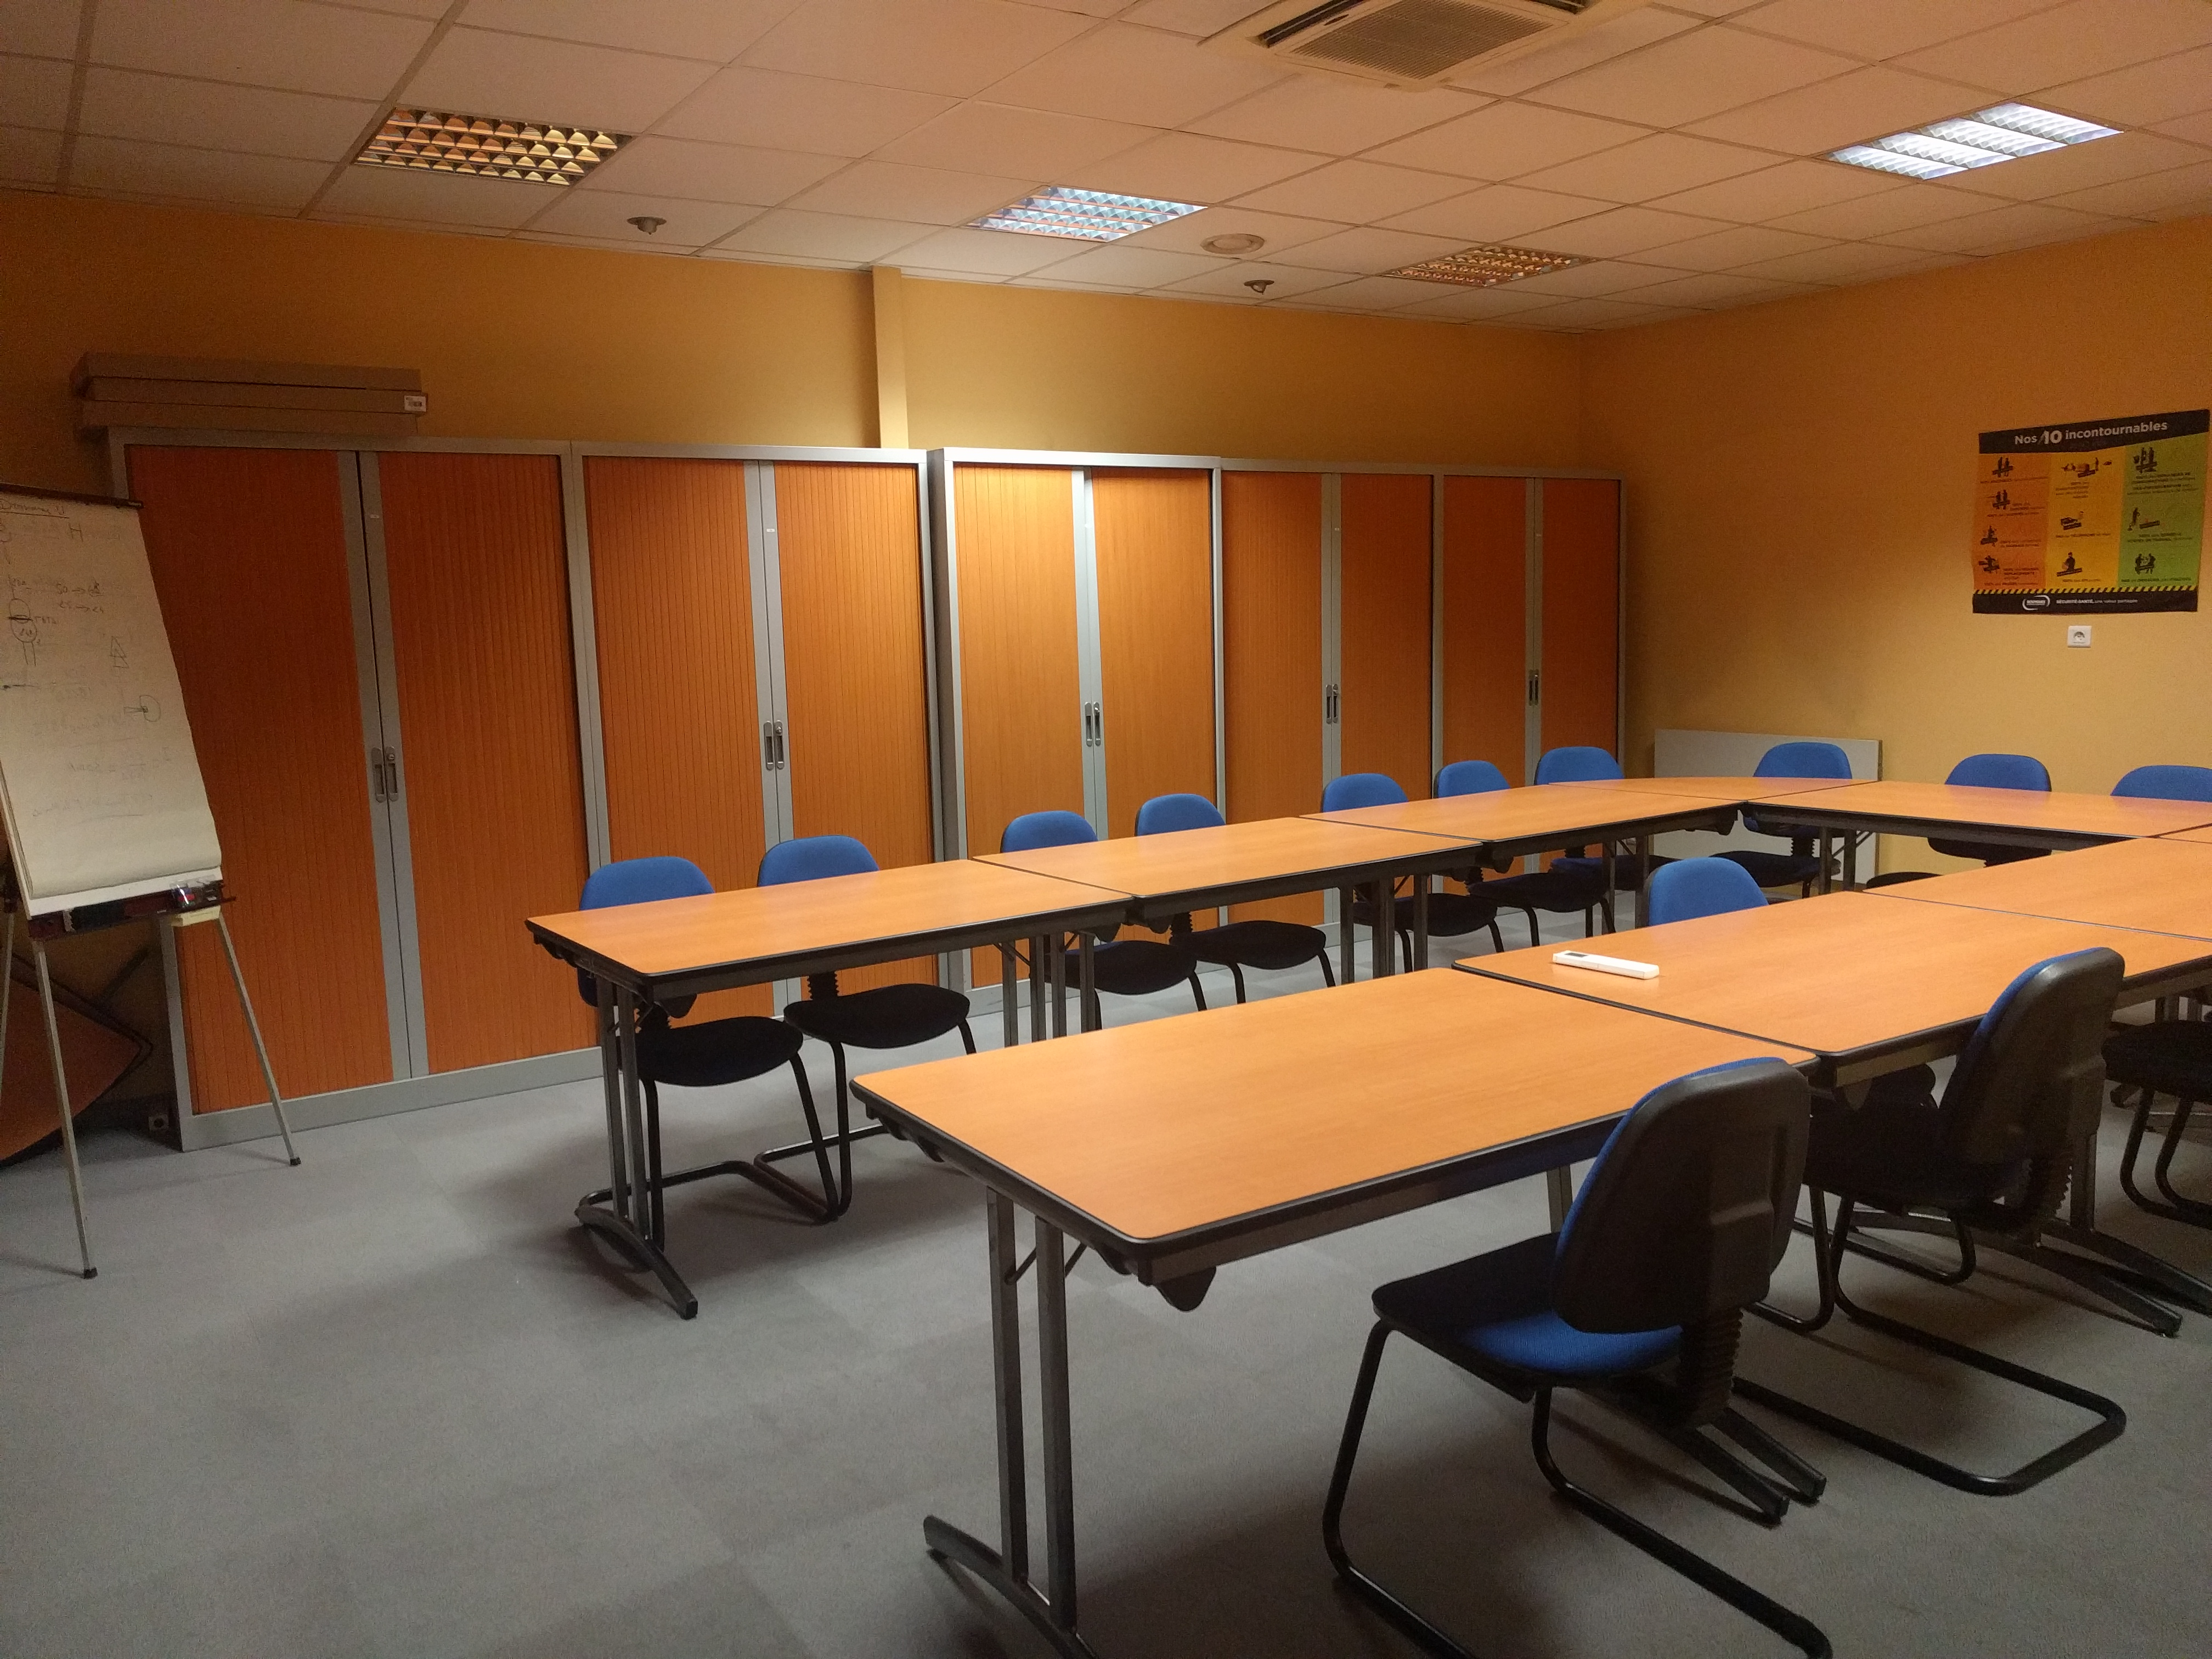
\includegraphics[scale=0.065]{img/salleReu}
        \caption{La grande salle de réunion des locaux}
    \end{figure}


    \subsection{Le personnel}

    Le groupe Bouygues entier emploie plus de 100 000 collaborateurs dont 44\% à l’international. Bouygues Energies et Services est une entreprise d'environ 3800 collaborateurs. \\

    Au sein des locaux dans lesquels j'ai travaillé dans le cadre de mon stage, nous étions environ 60 personnes (les effectifs varient d'une semaine sur l'autre du fait des différents projets en cours).  \\

    \begin{figure}[H]
        \centering
        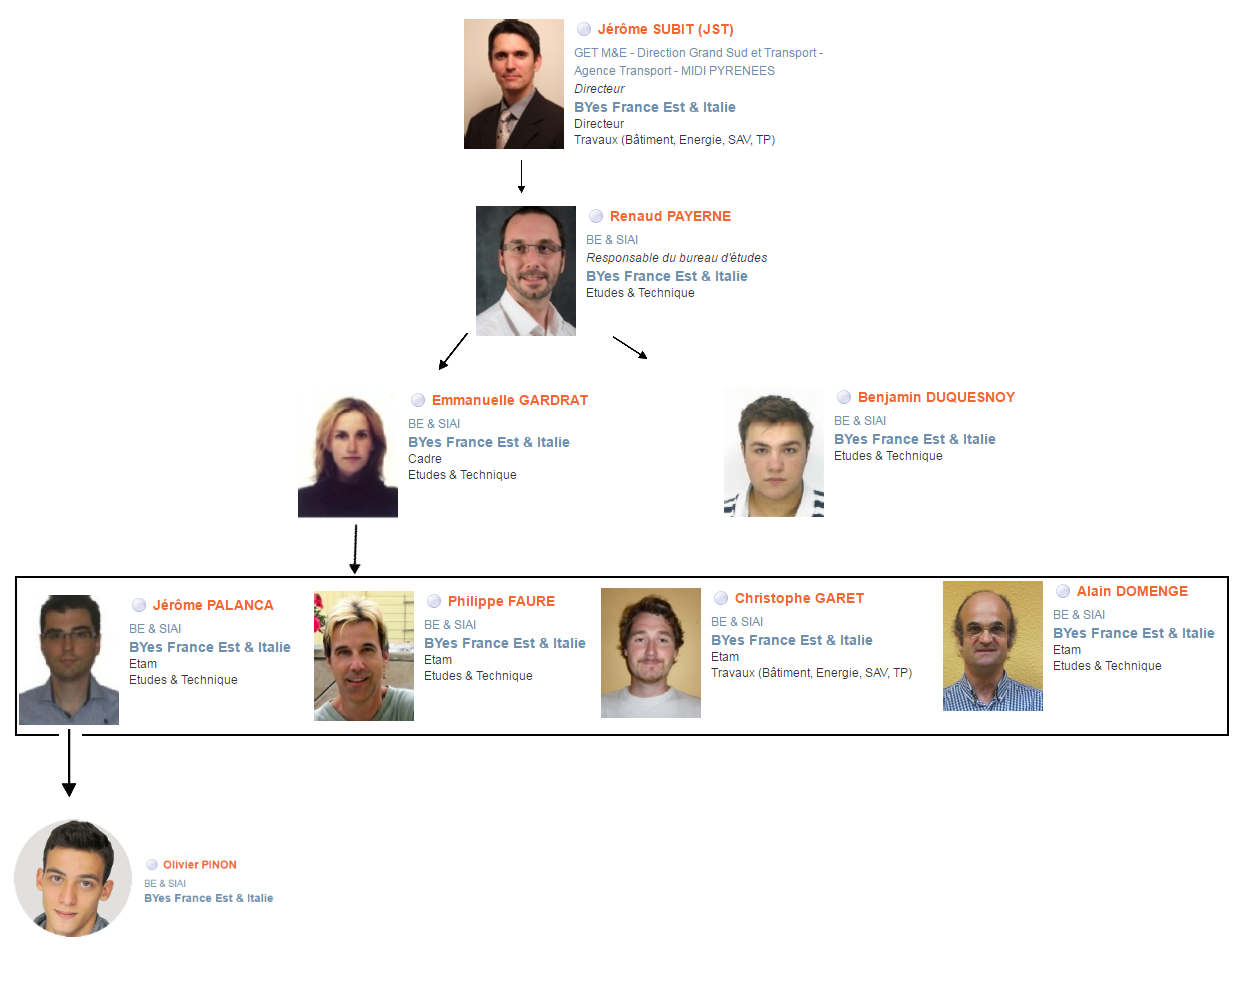
\includegraphics[scale=0.45]{img/Organigramme}
        \caption{Organigramme du bureau d'études de Bouygues Energies et Services - Annexe 1}
    \end{figure}

    Le service informatique n'est pas interne à l'entreprise. En effet, le groupe Bouygues a décidé de faire de l'IT Outsourcing\footnote{Avoir un parc informatique externe à l'entreprise, généralement géré par une entreprise tierce}, et donc de ne pas engager d'administrateur système dans le personnel de l'entreprise. La gestion informatique est donc effectuée par une autre filiale du groupe Bouygues, qui est appellée Structis. \\

    \subsection{L'équipe de travail}

    Durant la totalité de mon stage, j'ai travaillé en collaboration unique avec mon tuteur, Jérôme Palanca. Ce dernier n'ayant que peu de connaissances techniques sur l'utilisation des moteurs de jeu et le développement orienté objet, c'est lui qui se chargeait de la modélisation 3D des éléments, pendant que j'étais en charge de la conception objet et du développement réel de l'application. \\
    
    Le projet était effectué en parallèle du reste de l'activité du bureau d'études. J'ai eu une dizaine de collègues dans mon bureau de type open space, ce qui m'a permis de voir l'atmosphère de travail dans une équipe et de m'y habituer, mais tous mes collègues travaillaient sur des projets qui n'étaient pas en relation directe avec le mien. \\
    
    % Présentation du besoin
    \section{Le besoin de l'entreprise}
    \subsection{Le module d'habilitation éléctrique}

        L'habilitation éléctrique est un examen visant à certifier qu'un technicien est capable d'effectuer des opérations de maintenance sur un appareil fonctionnant sous haute tension, en restant dans les règles de sécurité mises en place. \\

        Cette habilitation est inhérente à chaque entreprise, et doit être effectuée par l'entreprise qui emploie le technicien pour être valide, même si l'idée reste globalement la même partout. \\

        C'est un examen d'une trentaine de minutes, qui est supervisé par un maître de formation qui fait passer chaque candidat à l'habilitation, un par un. De plus, l'examen nécéssite d'être effectué dans des conditions presques réelles avec des machines qui sont à la fois coûteuses et qu'il faut maintenir. \\

        \begin{figure}[H]
            \centering
            \includegraphics[scale=0.065]{img/localHabilitation}
            \caption{Le local d'habilitation vu de l'exterieur}
        \end{figure}

        \begin{figure}[H]
            \centering
            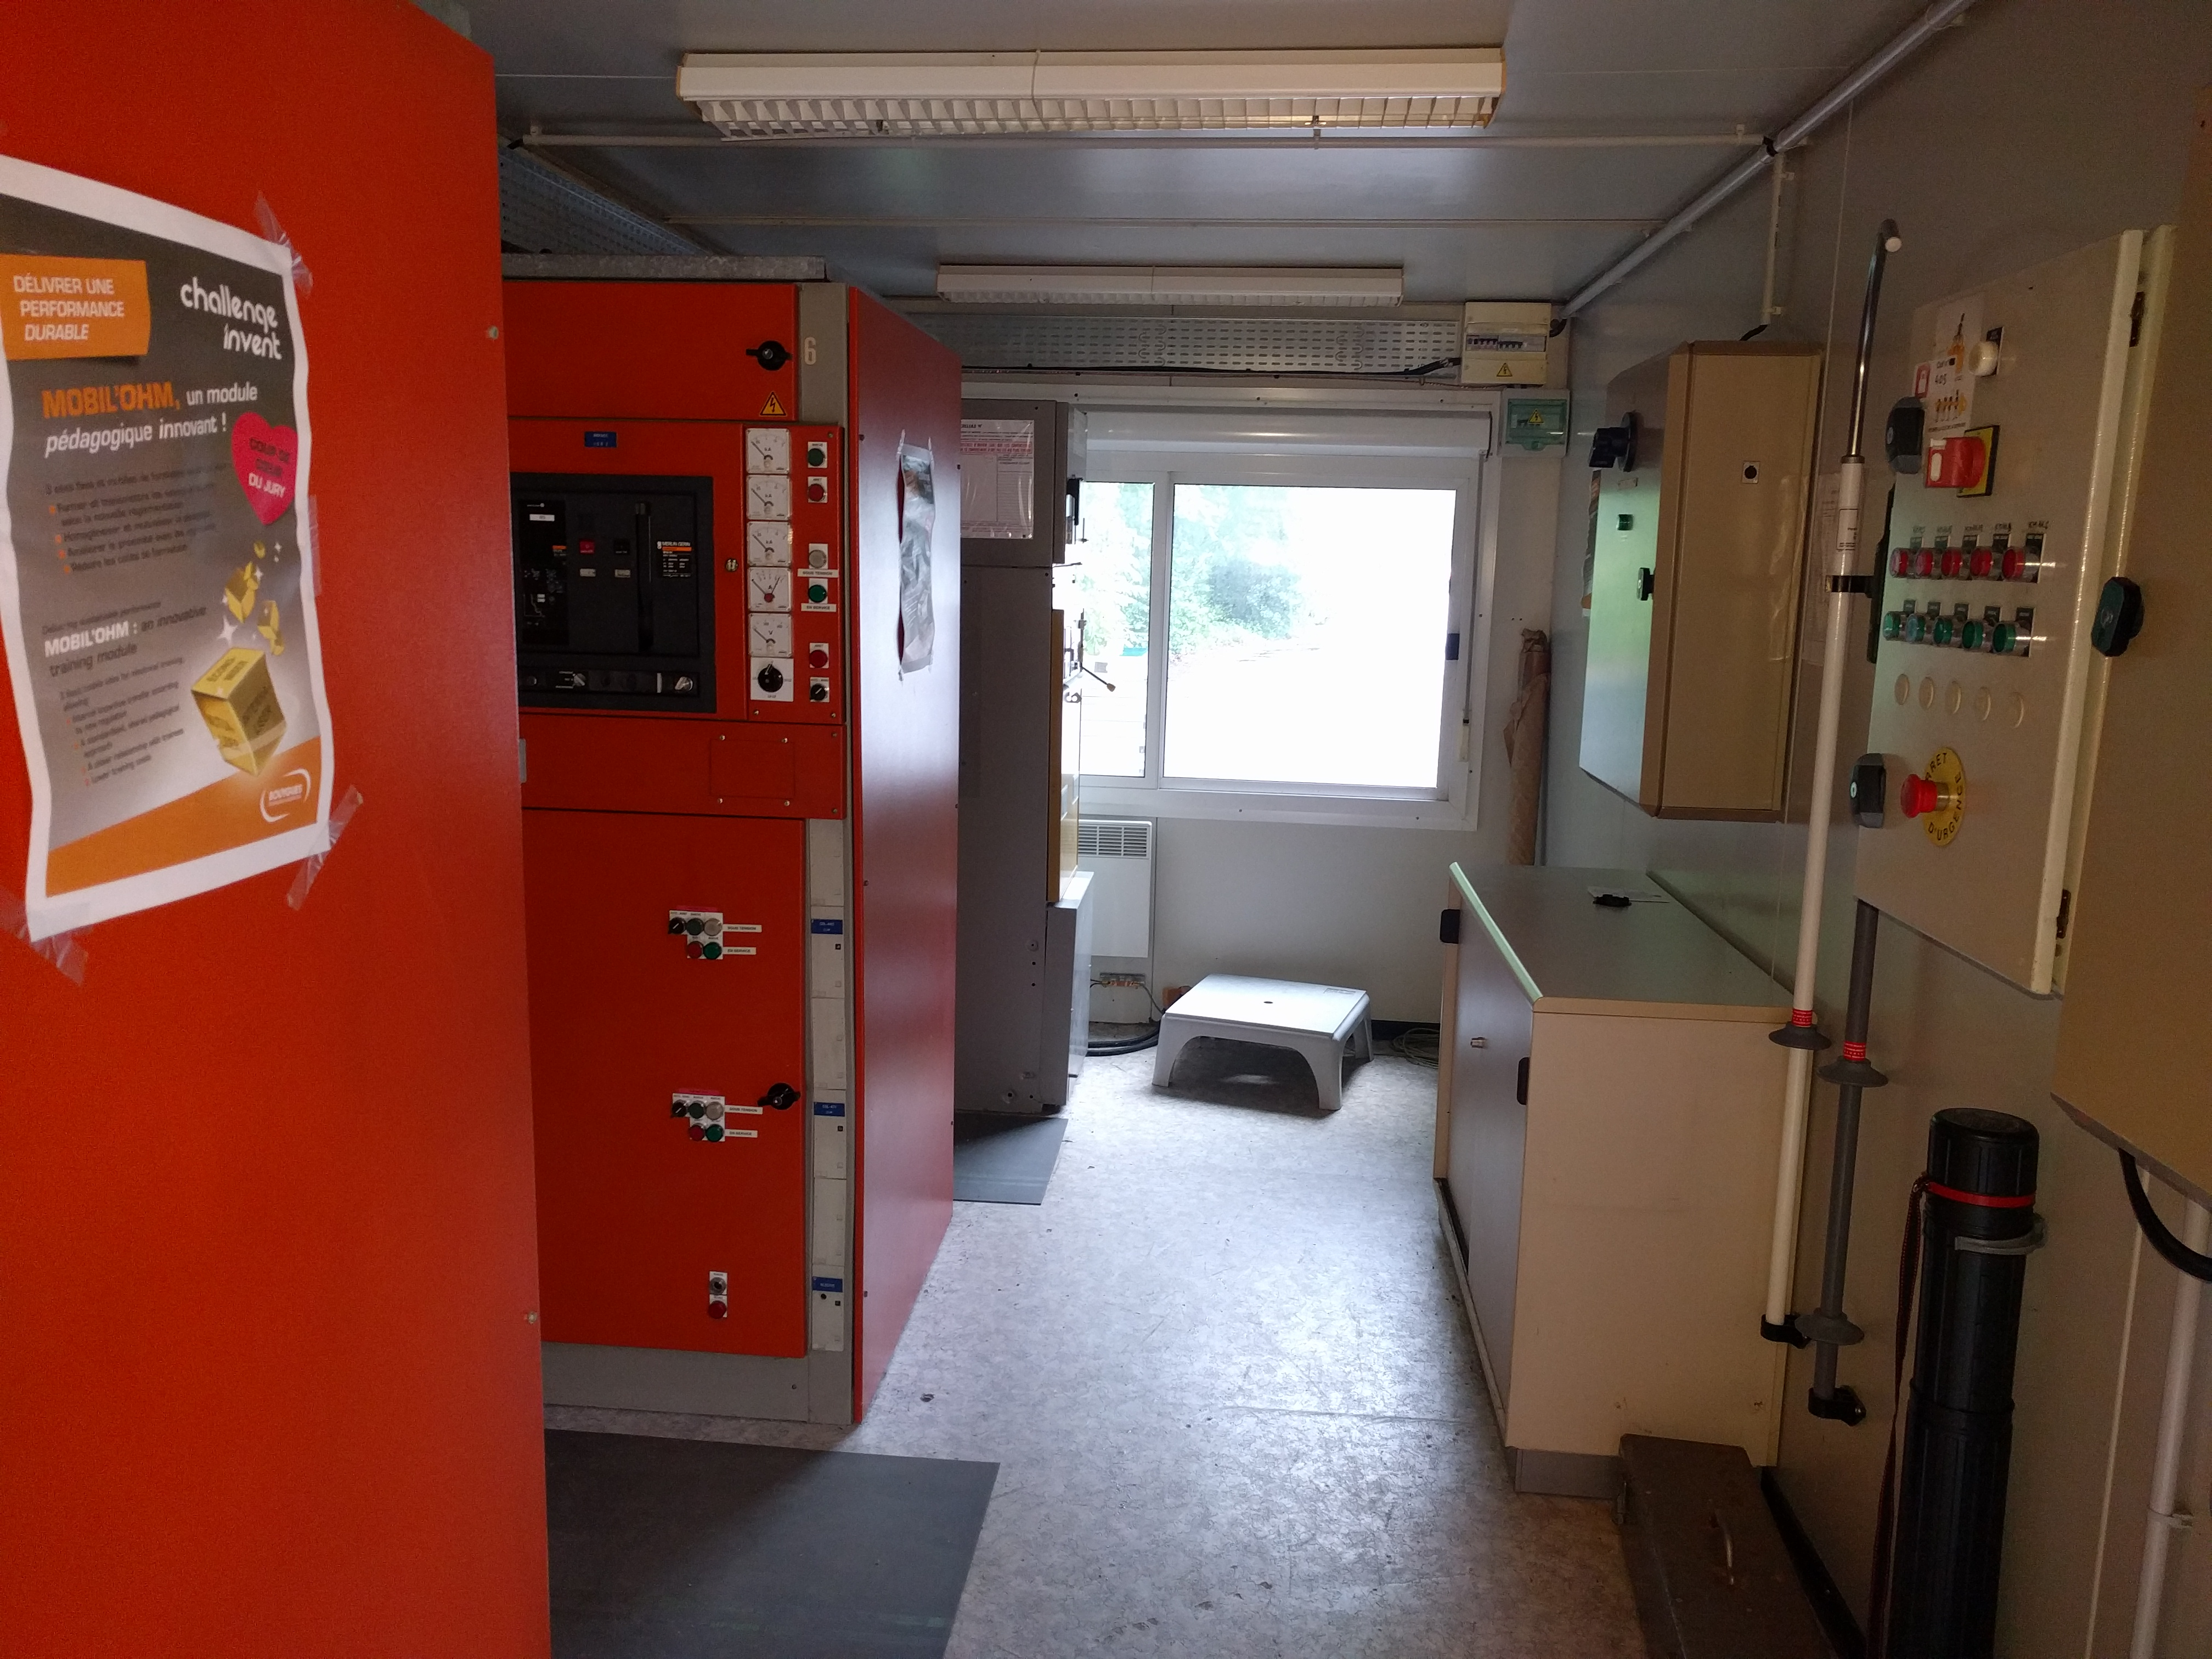
\includegraphics[scale=0.05]{img/habilitation1}
            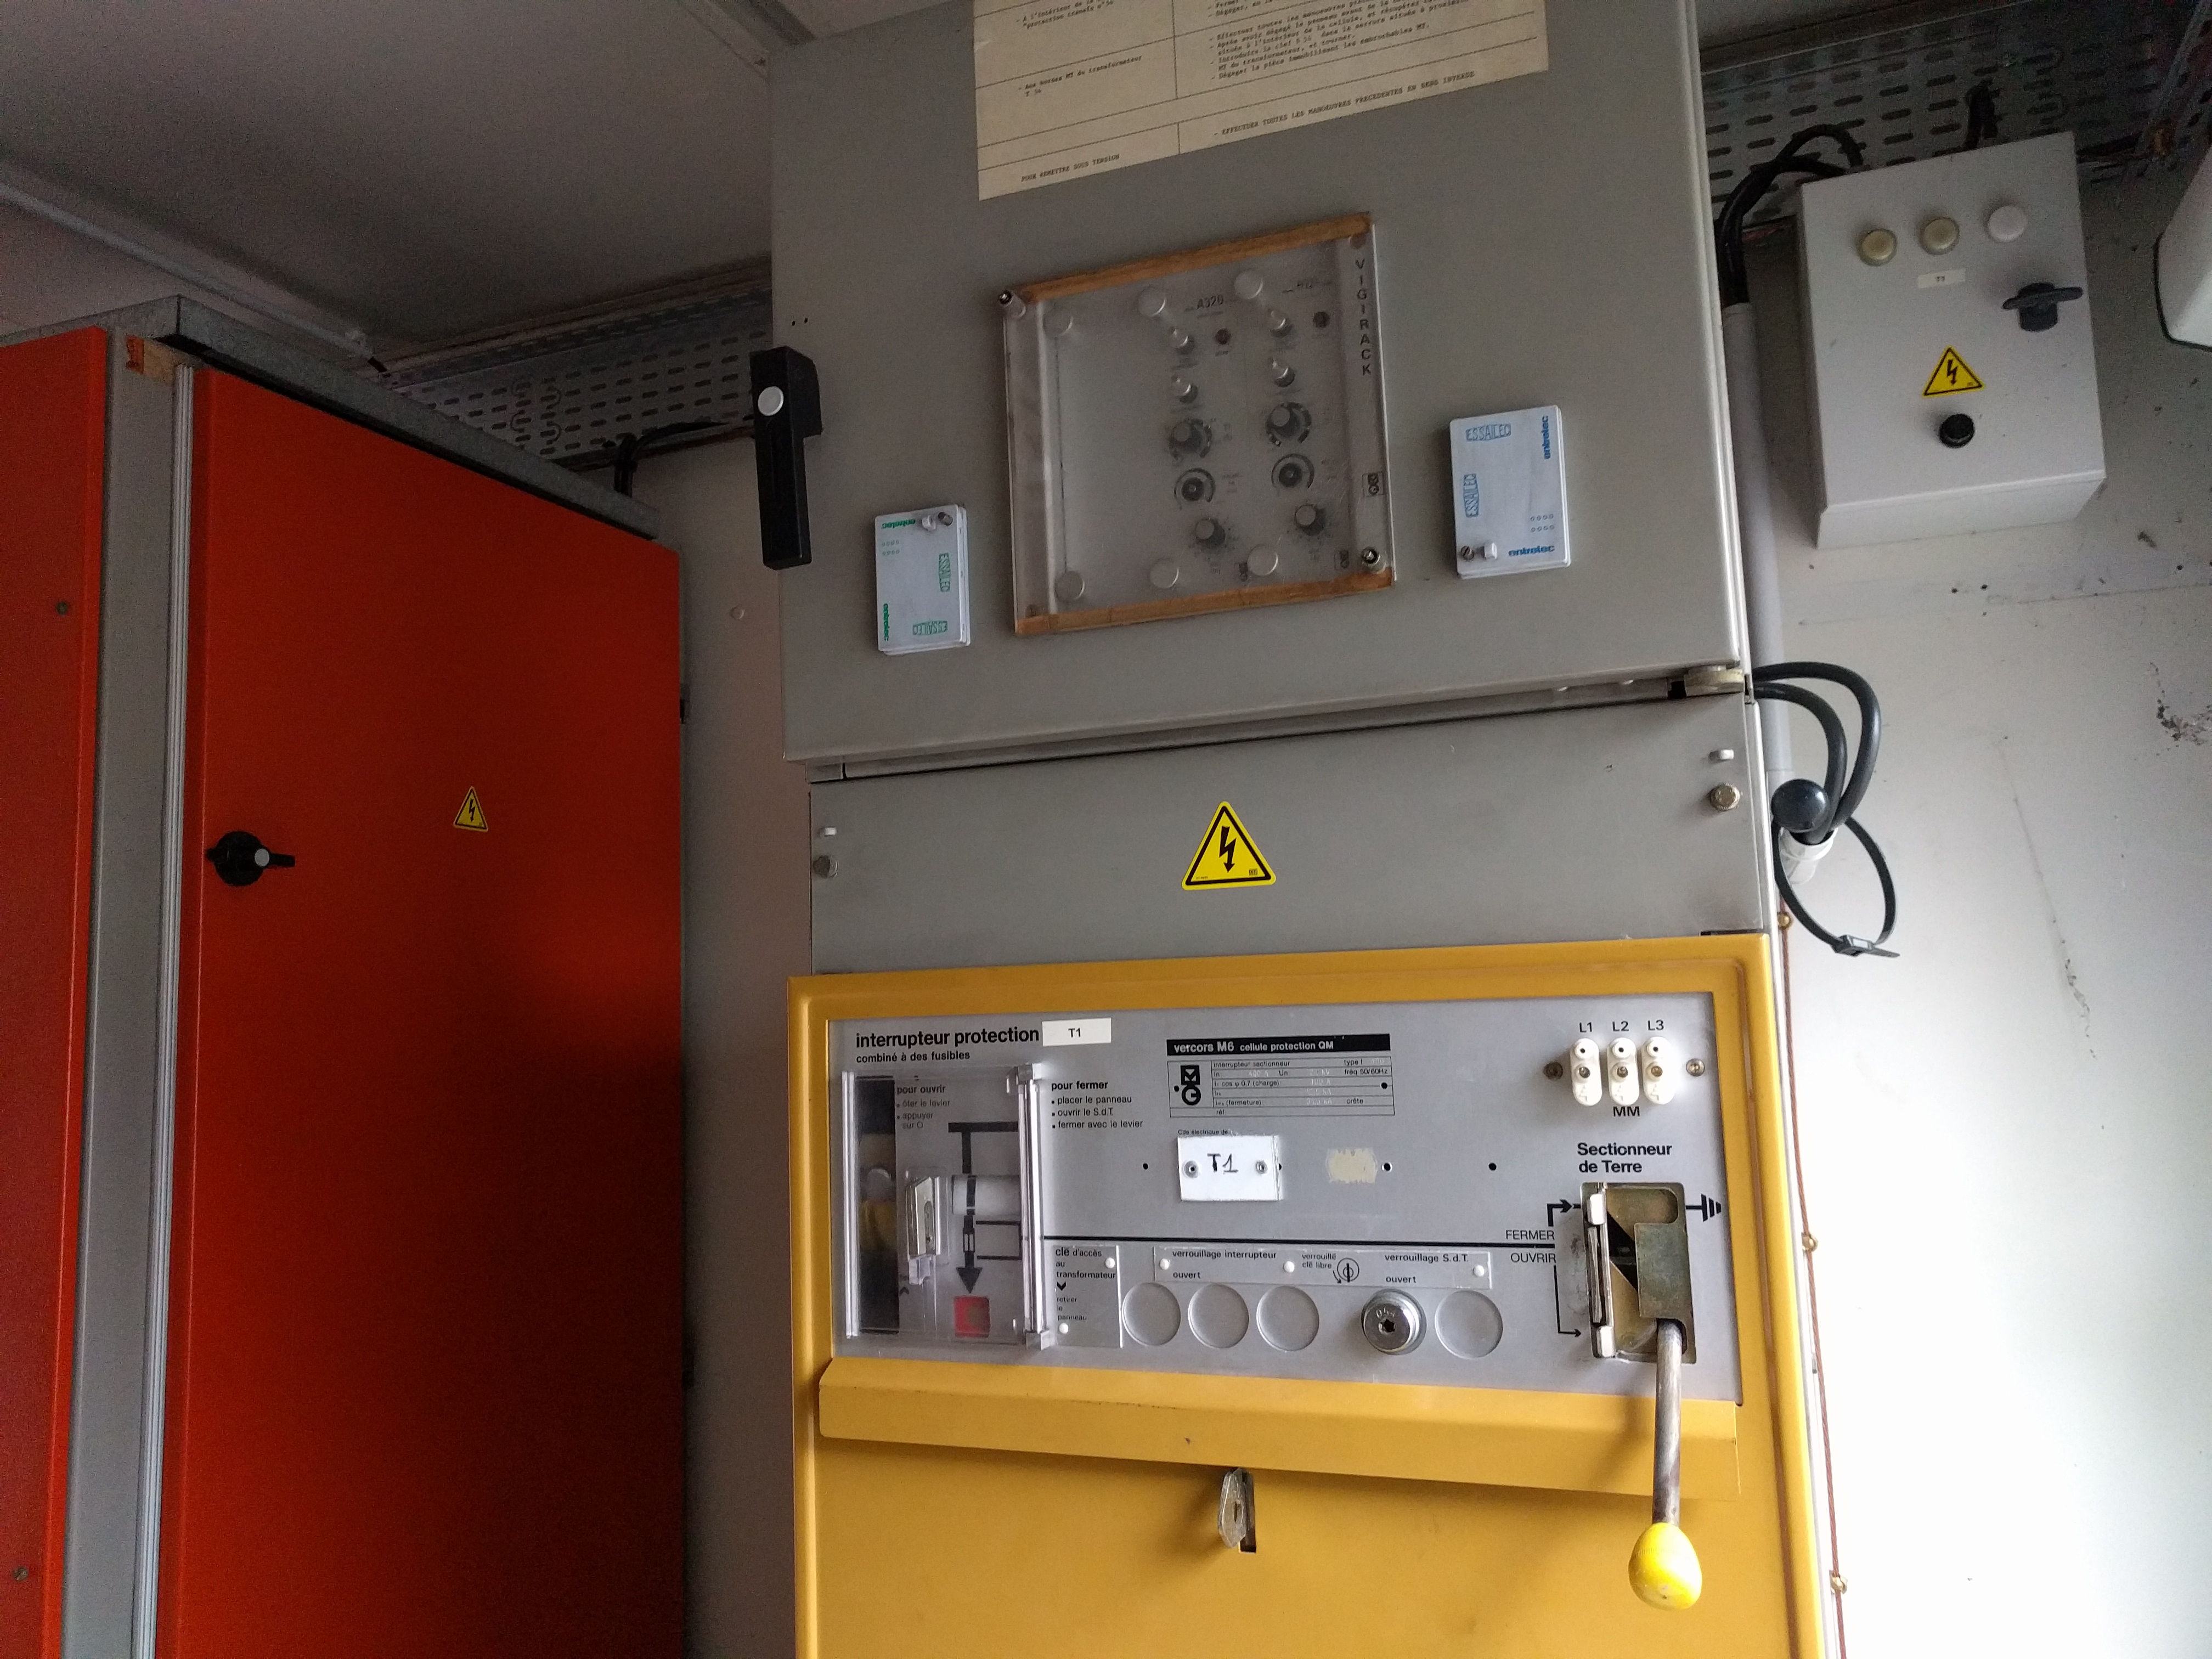
\includegraphics[scale=0.05]{img/habilitation2}
            \caption{Intérieur du local, deux machines sur lesquelles on effectue la formation}
        \end{figure}

        Cette habilitation peut être préparée par la lecture d'un manuel de préparation à l'habilitation électrique, dont on m'a confié un exemplaire dans le but de mieux appréhender les aspects techniques, et comprendre ce sur quoi j'allais travailler.

    \subsection{Le besoin d'un nouveau module}

        Le projet qui m'a été proposé est parti de Monsieur Renaud Payerne, et consiste à simuler cette formation avec la technologie de réalité virtuelle, non pas dans le but de remplacer cet examen obligatoire, mais plutôt d'en faciliter la formation. \\

        L'idée du projet est qu'en utilisant des technologies modernes rendant la chose plus ludique, les futurs habilités auront une formation de meilleure qualité. De plus, cette simulation permet de former plus de personnes à la fois, réduisant ainsi les moyens et le temps nécéssaire à l'habilitation. \\   

        De plus, le gros avantage de cette solution est la liberté qui est offerte au formateur de pouvoir montrer l'intérieur des machines aux futurs habilités. De cette façon, la compréhension du formé est favorisée par la vision des éléments qui l'entourent. \\

    \subsection{Les fonctionnalités de l'application}

    Durant la réalisation du projet, aucun listing de fonctionnalités préalable n'a été fait, car cela nécéssitait trop de temps. L'application en elle-même vise à démontrer l'efficacité et l'intérêt d'un nouveau module d'habilitation éléctrique, qui est à perfectionner. Nous pouvons cependant effectuer une analyse rétrospective de l'application, et définir les acteurs principaux du système et les actions qu'ils peuvent effectuer dans la simulation. \\

    \begin{figure}[H]
        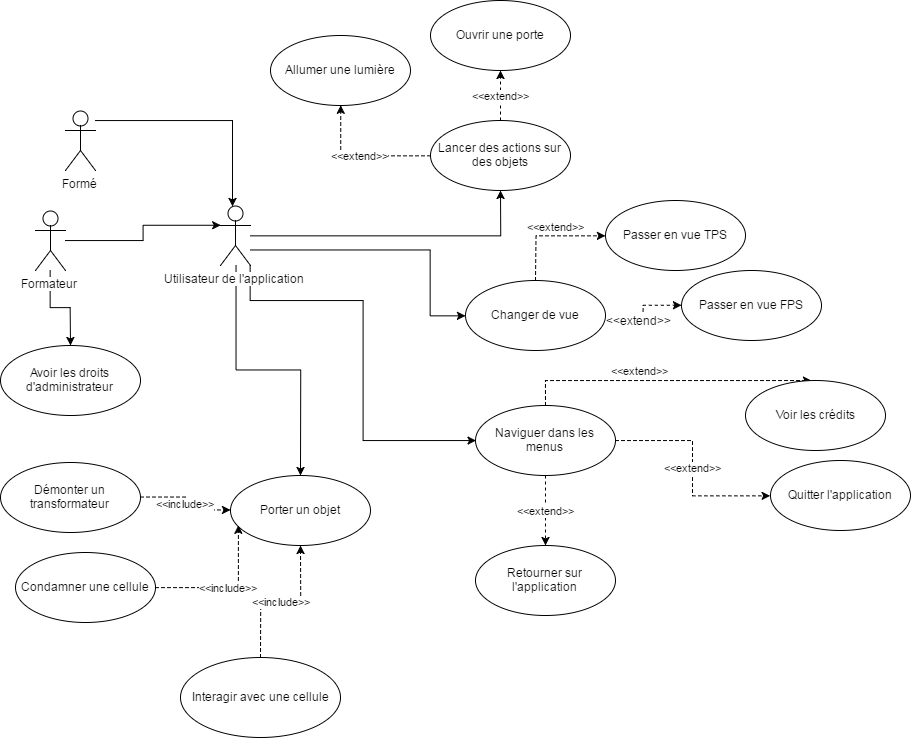
\includegraphics[scale=0.5]{img/UseCases}
        \caption{Diagramme de cas d'utilisation de l'application - Annexe 2}
    \end{figure}

    \subsection{Les solutions utilisées}

    Le choix des moyens techniques a été réalisé en amont de mon stage par l'équipe qui a lancé le projet au bureau d'étude de Bouygues Energies et Services. \\ 

    Afin de développer l'application, nous avons choisi d'utiliser le moteur de jeu Unity, pour les performances, la rapidité de développement, la polyvalence et la modularité qui est la sienne. De plus, nous avons pu utiliser des licences gratuites, car l'utilisation que nous avons du moteur n'est pas commerciale. L'utilisation d'un autre moteur, comme Unreal, ne nous a pas paru être un bon choix, notamment parce qu'il nécéssite des compétences en C++, qui n'est pas dans les langages que je maîtrise parfaitement. \\

    \begin{figure}[H]
        \centering
        
\includegraphics[scale=0.5]{img/logo-unity}
        \hspace{10pt}
        
\includegraphics[scale=0.5]{img/logo-unreal}
        \caption{Unity / Unreal Engine}
    \end{figure}

    Bien que j'eusse préféré utiliser Linux comme environnement de développement, j'ai eu à travailler sur Windows car les ordinateurs fournis par Structis tournent uniquement sur ce système d'exploitation. Le principal avantage que j'ai eu en utilisant Windows a été de ne pas avoir eu à me soucier de la compatibilité entre les différents systèmes d'exploitations, même si Unity gère ce problème de façon transparente. \\

    \begin{figure}[H]
        \centering
        
\includegraphics[scale=0.5]{img/logo-w10}
        \hspace{10pt}
        
\includegraphics[scale=0.5]{img/logo-linux}
        \caption{Windows 10 / Linux}
    \end{figure}
    
    Le language C\# a été utilisé pour le scripting de l'application elle-même, puisque c'est celui que j'avais personnellement le plus utilisé avec le moteur de jeu, je connaissais donc bien l'API\footnote{Application Programming Interface, interface permettant de développer en utilisant un logiciel ou une solution depuis un language de programmation}. De plus, il existe de nombreux comparatifs de performance entre JavaScript et C\#, qui montrent qu'une application développée avec l'API que nous avons utilisé sera bien plus performante. \\

    \begin{figure}[H]
        \centering
        
\includegraphics[scale=0.35]{img/logo-csharp}
        \hspace{10pt}
        
\includegraphics[scale=0.75]{img/logo-javascript}
        \caption{C\# / JavaScript}
    \end{figure}

    Le choix de l'IDE\footnote{IDE : Integrated Development Environment, EDI en Français, se dit d'un logiciel contenant une suite d'outils permettant de développer dans un language informatique} que j'ai utilisé, Visual Studio Code, a été fait suite à une recommendation de mon tuteur, que j'ai approuvé puisque beaucoup de mes collègues à l'IUT m'avaient déjà proposé d'apprendre à l'utiliser. Cet outil très puissant, extrêmement modulable, et adapté au développement pour Unity a été une des très bonne découvertes que j'ai pu faire durant mon stage, et je l'utilise désormais comme mon IDE pour tous les languages dans mes projets personnels. Nous avons volontairement décidé de ne pas utiliser Visual Studio pour Windows ; Ce logiciel aurait coûté une licence en plus pour mon projet car Bouygues Energies et Services fait plus d'un million d'euros de chiffre d'affaires, et que j'ai personnellement préféré apprendre à utiliser une technologie que je n'avais pas encore utilisé. \\

    \begin{figure}[H]
        \centering
        
\includegraphics[scale=0.05]{img/Logo-VSCode}
        \hspace{10pt}
        
\includegraphics[scale=0.5]{img/logo-visual-studio}
        \caption{Visual Studio Code / Visual Studio}
    \end{figure}

    Pour la modélisation 3D, nous avons choisi d'utiliser SketchUp, car c'est le logiciel que mon tuteur savait utilisé, et qu'il est très facile à prendre à main, j'ai donc également pu m'essayer au dessin assisté par ordinateur, par exemple en m'exerçant à reproduire un BAPI\footnote{BAPI : Bloc Autonome Portatif d'Intervention, sorte de grosse lampe torche que l'on trouve dans les sous-stations} dans le logiciel SketchUp avant de l'importer sous Unity \\

    \begin{figure}[H]
        \centering
        
\includegraphics[scale=0.5]{img/Logo-skp}
        \caption{Google SketchUp}
    \end{figure}

    \begin{figure}[H]
        \centering
        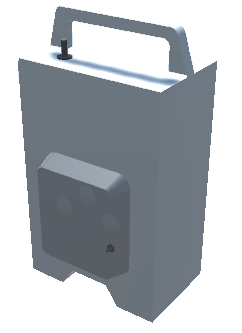
\includegraphics[scale=0.5]{img/BAPI-Screen}
        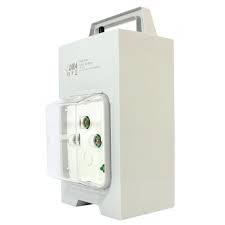
\includegraphics[scale=0.5]{img/BAPI-Reel}
        \caption{Ma représentation 3D d'un BAPI / Un vrai BAPI}
    \end{figure}

    % Etude et réalisation
    \section{Etude et réalisation de l'application}

    \subsection{La gestion de projet}
    
     Dans le cadre du projet, nous avons choisi un cycle de développement suivant une méthode agile, très comparable à la méthode Scrum. Pour cette raison, il n'a pas été possible de faire un diagramme de Gantt pour la gestion des tâches en début de projet. Voici alors le diagramme de Gantt\footnote{Diagramme retrospectif, dans ce cas} de la planification des tâches du projet :

     \begin{figure}[H]
        \centering 
        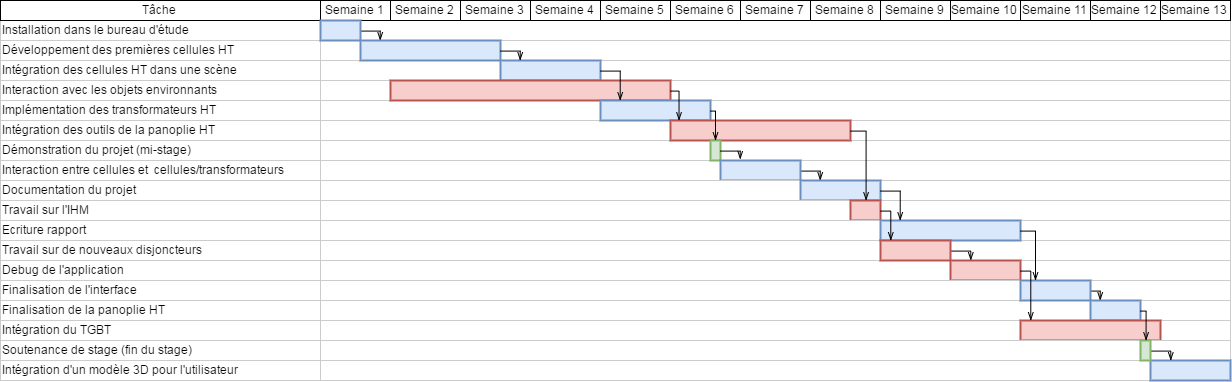
\includegraphics[scale=0.375]{img/GanttStage}
        \caption{Diagramme de Gantt - planification des tâches du stage - Annexe 1}
     \end{figure}

     Légende du diagramme : 
     \begin{itemize}
        \item Les tâches bleues sont les tâches principales du projet \\
        \item Les tâches rouges sont les tâches secondaires, réalisées en parallèles\\
        \item Les tâches vertes sont les évènements du projet qui marquent le milieu et la fin du stage \\
     \end{itemize}

     Afin de suivre une certaine trame dans le développement du projet, mon tuteur de stage a mis en place dès le début du stage un Trello, sur lequel il mettait les différentes tâches que j'avais à remplir pour avancer dans le développement, ainsi que différentes indications me permettant de mieux comprendre ce que j'avais à reproduire. En plus de cela, mon tuteur marquait ses propres tâches afin que nous puissions synchroniser nos travaux. Voici deux captures d'écrans qui montrent l'évolution du Trello durant le projet. \\

     \begin{figure}[H]
        \centering
        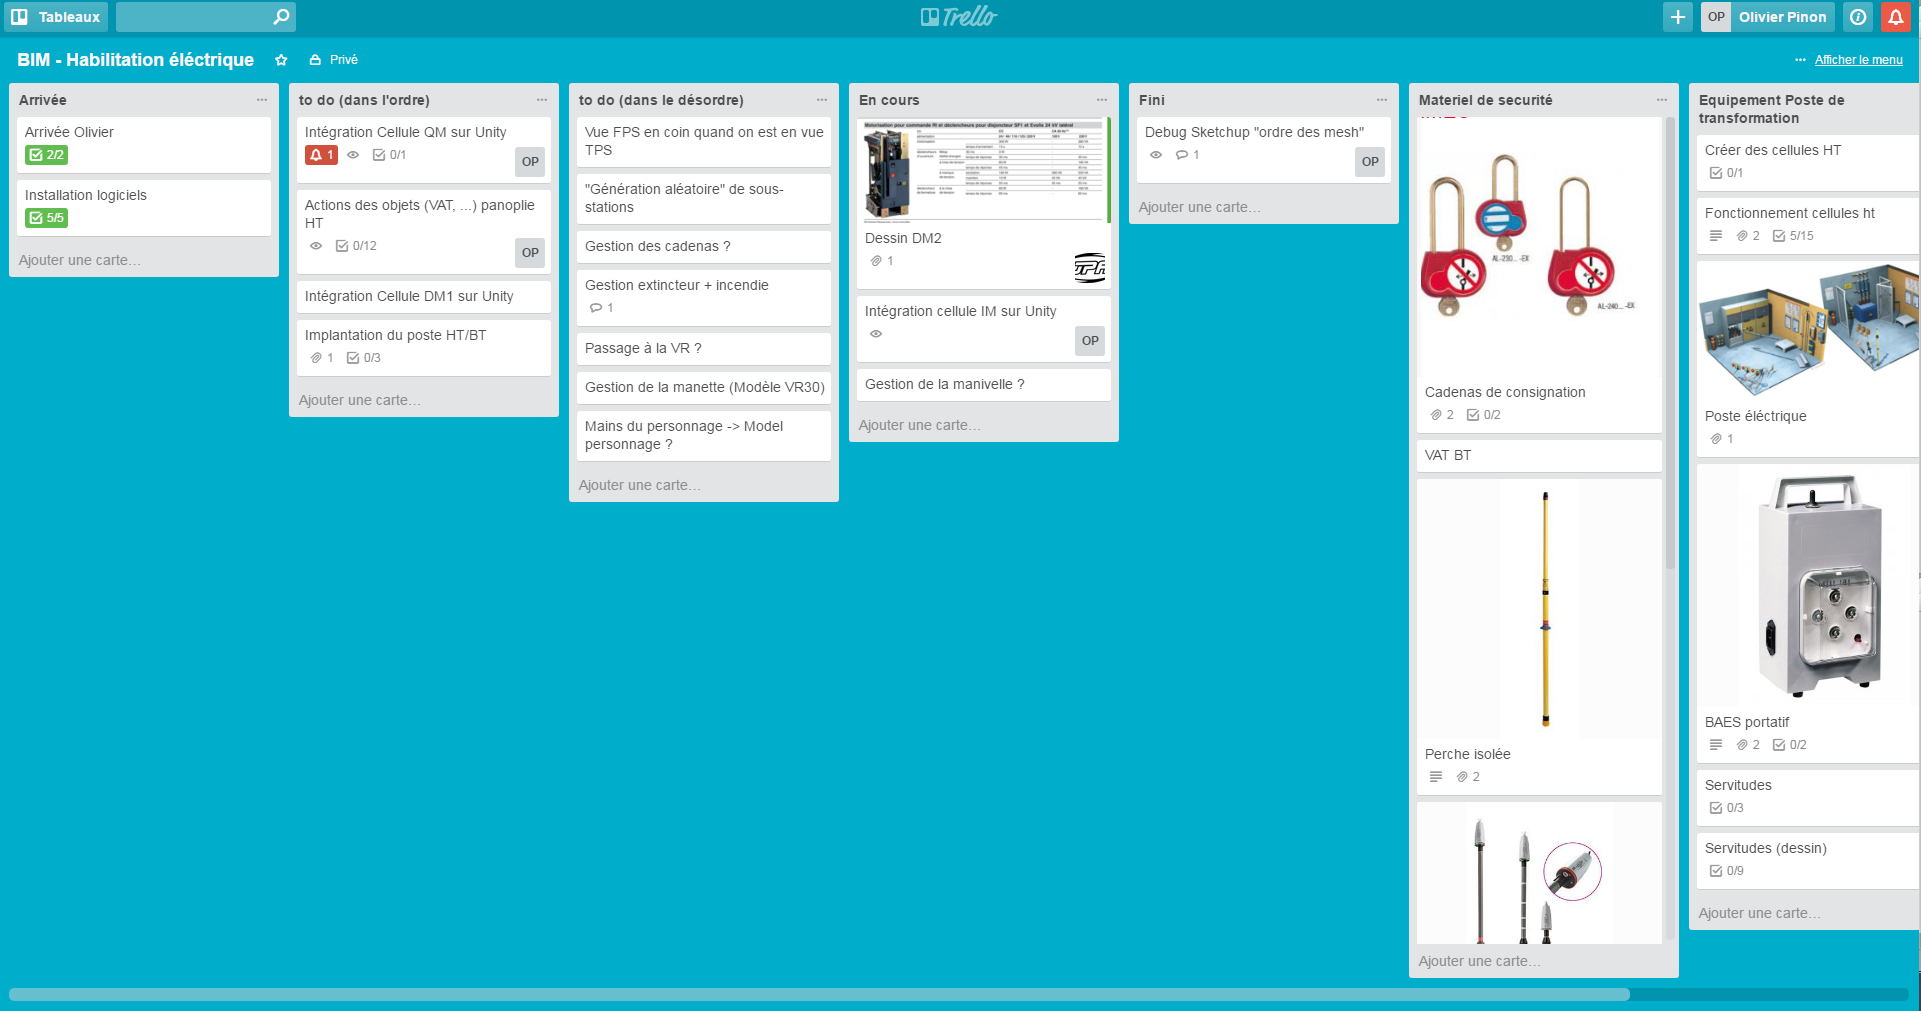
\includegraphics[scale=0.15]{img/trello1}
        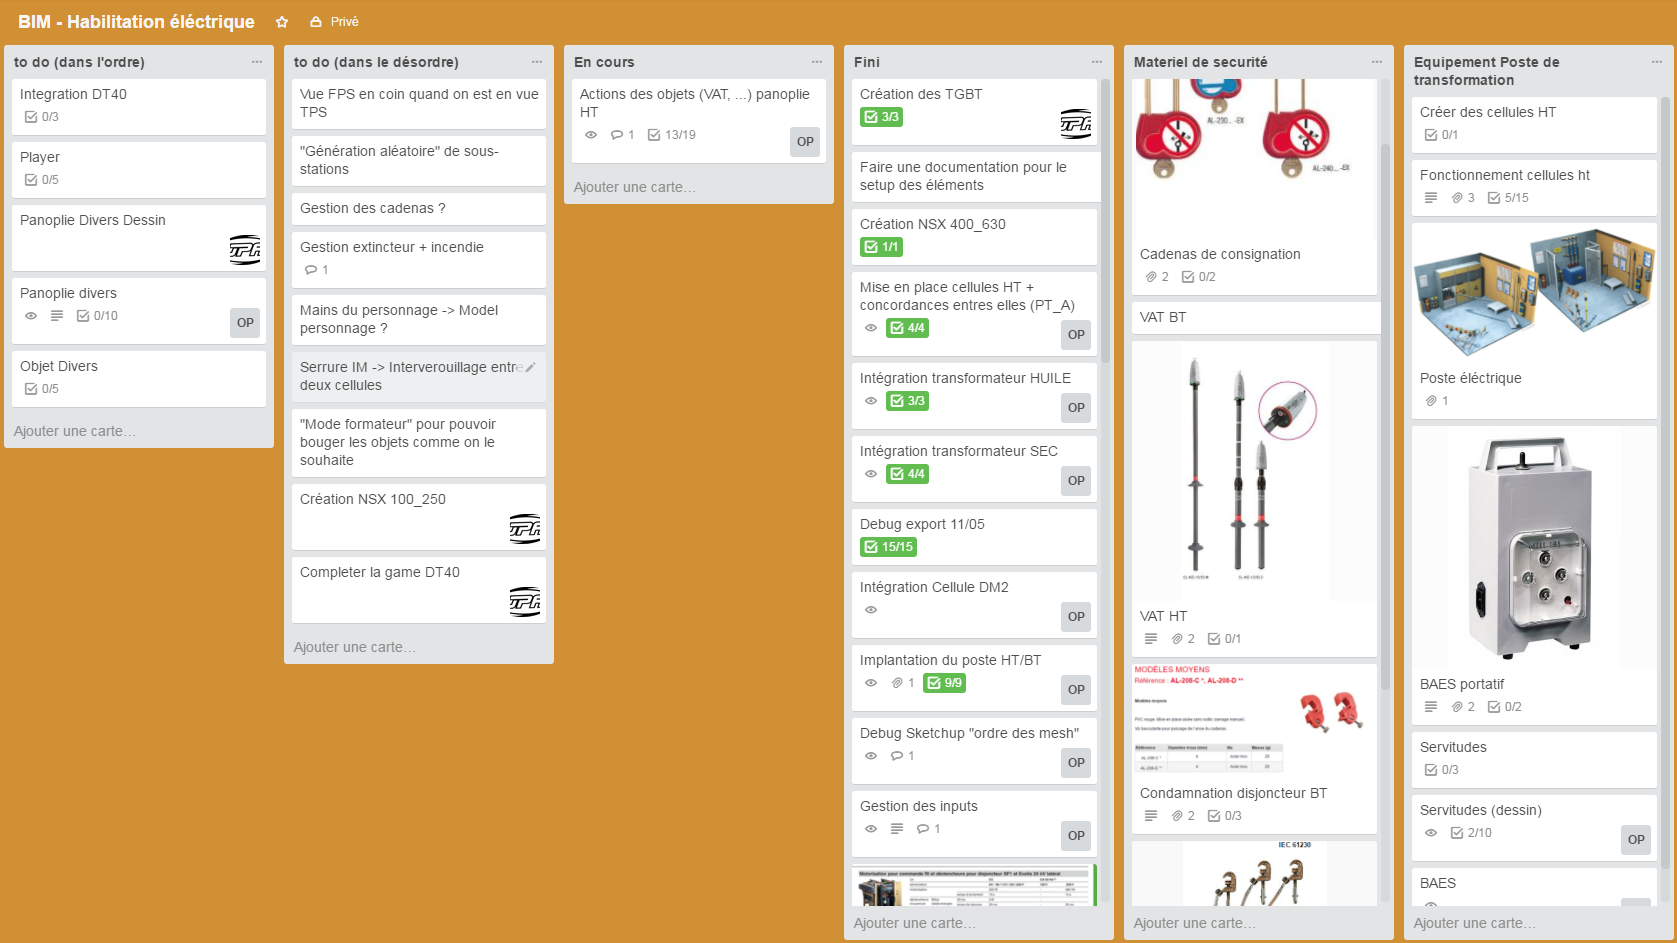
\includegraphics[scale=0.15]{img/trello2}
        \caption{Etat du Trello - 19 Avril 2017 / 29 Mai 2017 - Annexes 1 et 2}
     \end{figure} 

    \subsection{Conception du projet}

    \subsubsection{Le problème de la conception objet}

    La plus grosse difficulté du projet, à mon goût, a été de suivre le cycle de développement agile que nous avons mis en place, sans avoir constitué un réel cahier des charges au début du stage. La trame Trello mise en place ne permettait pas de définir une conception objet valable. En effet, même si mon tuteur m'a souvent dit de \"voir loin\" pour le développement, pour chaque partie du système, il était possible que le besoin, que je ne pouvais pas prévoir, change d'une heure sur l'autre. La phase de conception a donc été très compliquée pour moi et a entraîné du retard sur la phase de réalisation. \\
    
    Chaque fois qu'un nouveau problème m'était posé, je prenais du temps pour effectuer un croquis, sorte de schéma semblable à de l'UML. Une fois cette première réflexion effectuée, je faisais valider le principe par mon tuteur afin qu'il comprenne comment j'allais résoudre le problème. Je procédais ensuite à la réalisation d'un diagramme UML (très souvent un diagramme de classe). Pour la réalisation des cellules et transformateurs haute tension, qui ont un fonctionnement bien précis, il a été fréquent que je réalise un diagramme d'état-transitions. \\ 

    \subsubsection{Utilisation du moteur de jeu Unity}

    Afin de comprendre la conceptualisation objet que j'ai effectué, il faut tout d'abord comprendre le principe d'Unity. \\

    Unity est un moteur de jeu ; C'est un ensemble de composants logiciels qui permet d'effectuer une simulation en temps réel. Ce type d'outil prend en charge toutes les différentes couches à notre place, rendant le développement de notre module plus facile. Notamment, Unity va gérer pour nous : \\
    
    \begin{itemize}

        \item Le moteur graphique, qui permet d'afficher des formes géométriques 2D et 3D à l'écran, avec toutes les textures, les animations, et les fioritures graphiques qui y sont associées. \\

        \item Le moteur son, qui permet de gérer la spatialisation audio, afin d'immerger l'utilisateur dans un univers sonore. \\
 
        \item Le moteur logique, qui permet de gérer le déroulement d'une application, du lancement à l'extinction du processus, en assurant tout le temps un nombre d'images par seconde précis. C'est le chef d'orchestre qui permet l'harmonisation entre les autres moteurs. \\

        \item Le moteur physique, qui gère les déplacements, la gravité, les collisions entre éléments, tout ce qui est régi par les lois de la physique. \\

        \item Le moteur réseau, qui permet de synchroniser les actions entre différentes applications par l'intermédiaire d'un programme agissant comme un serveur. \\

        \item Le moteur d'intelligence artificielle, qui permet de gérer la prise de décision relative à chaque entité présente dans la simulation. \\
    \end{itemize}

    Utiliser un moteur de jeu se fait le plus souvent par l'intermédiaire de son éditeur approprié. On va ensuite pouvoir ajouter des objets dans une scène, et gérer leur comportement face aux différentes actions de l'utilisateur grâce à des scripts écrits utilisant l'API du moteur de jeu. \\

    \begin{figure}[H]
        \centering
        \caption{Exemple de mon environnement de travail quotidien}
    \end{figure}

    Techniquement parlant, Unity se base sur un Design Pattern\footnote{Patron de conception en français, solution éprouvée pour résoudre un problème d'architecture logicielle} que l'on apelle EC\footnote{Entity Component}, qui s'inspire du design pattern ECS\footnote{Entity Component System}. Sur Unity, la couche \"System\" est gérée automatiquement, et n'est pas directement modifiable par l'utilisateur. Ce design pattern peut être représenté par le diagramme de classe suivant. \\

    \begin{figure}[H]
        \centering
        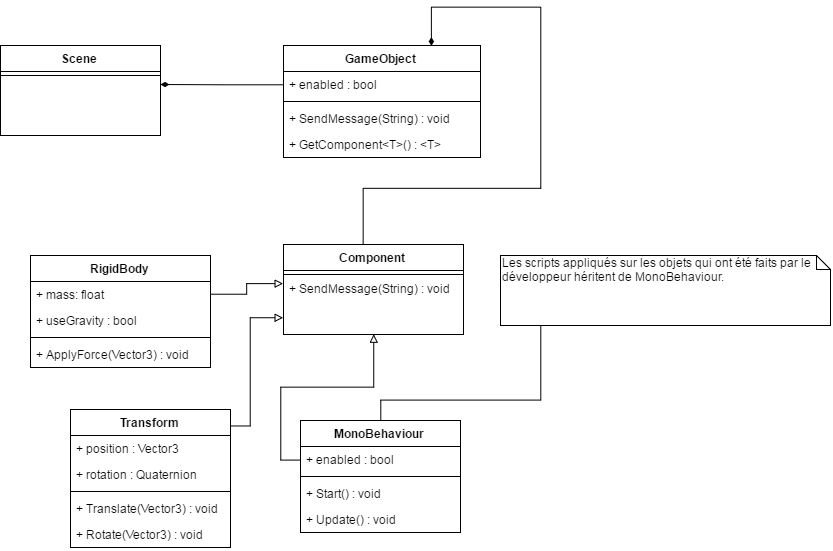
\includegraphics[scale=0.45]{img/DiagClasseEntityComponent}
        \caption{Représentation simplifiée du Design Pattern \"Entity Component\" - Annexe 10}
    \end{figure} 

    Quand on utilise Unity, on crée des classes qui héritent de MonoBehaviour, qui représentent pour le moteur de jeu un composant écrit en C\#. Il est donc impliqué dans tous les diagrammes UML suivant que ces scripts héritent de MonoBehaviour. \\

    Par nature, l'utilisation du moteur de jeu nous pousse à rendre tous nos attributs publics afin de rendre l'utilisation et la communication entre les composants plus facile. \\

    \subsubsection{Conceptualisation des systèmes}

    \paragraph{Le système de cellules}

    Les premiers éléments qui ont été reproduits dans la simulation sont les cellules à haute tension. Une cellule est à la fois une source d'énergie et prend sa source d'énergie sur une cellule. Chaque cellule HT est spéciale et définie dans la documentation du projet. \\

    Chaque cellule a sa propre implémentation des fonctions d'animations, car les cellules ne fonctionnent pas toutes selon le même schéma. Certaines ont des disjoncteurs, d'autres ont seulement des interupteurs, voire aucun des deux. \\

    Pour la simulation, il a été défini un type de cellule spéciale, nommée arrivée EDF. Cette dernière représente le courant délivré, qui alimente en continu. Il faut noter que cette arrivée peut être coupée, afin que le formateur puisse simuler une coupure de courant pendant l'intervention. \\

    \begin{figure}[H]
        \centering
        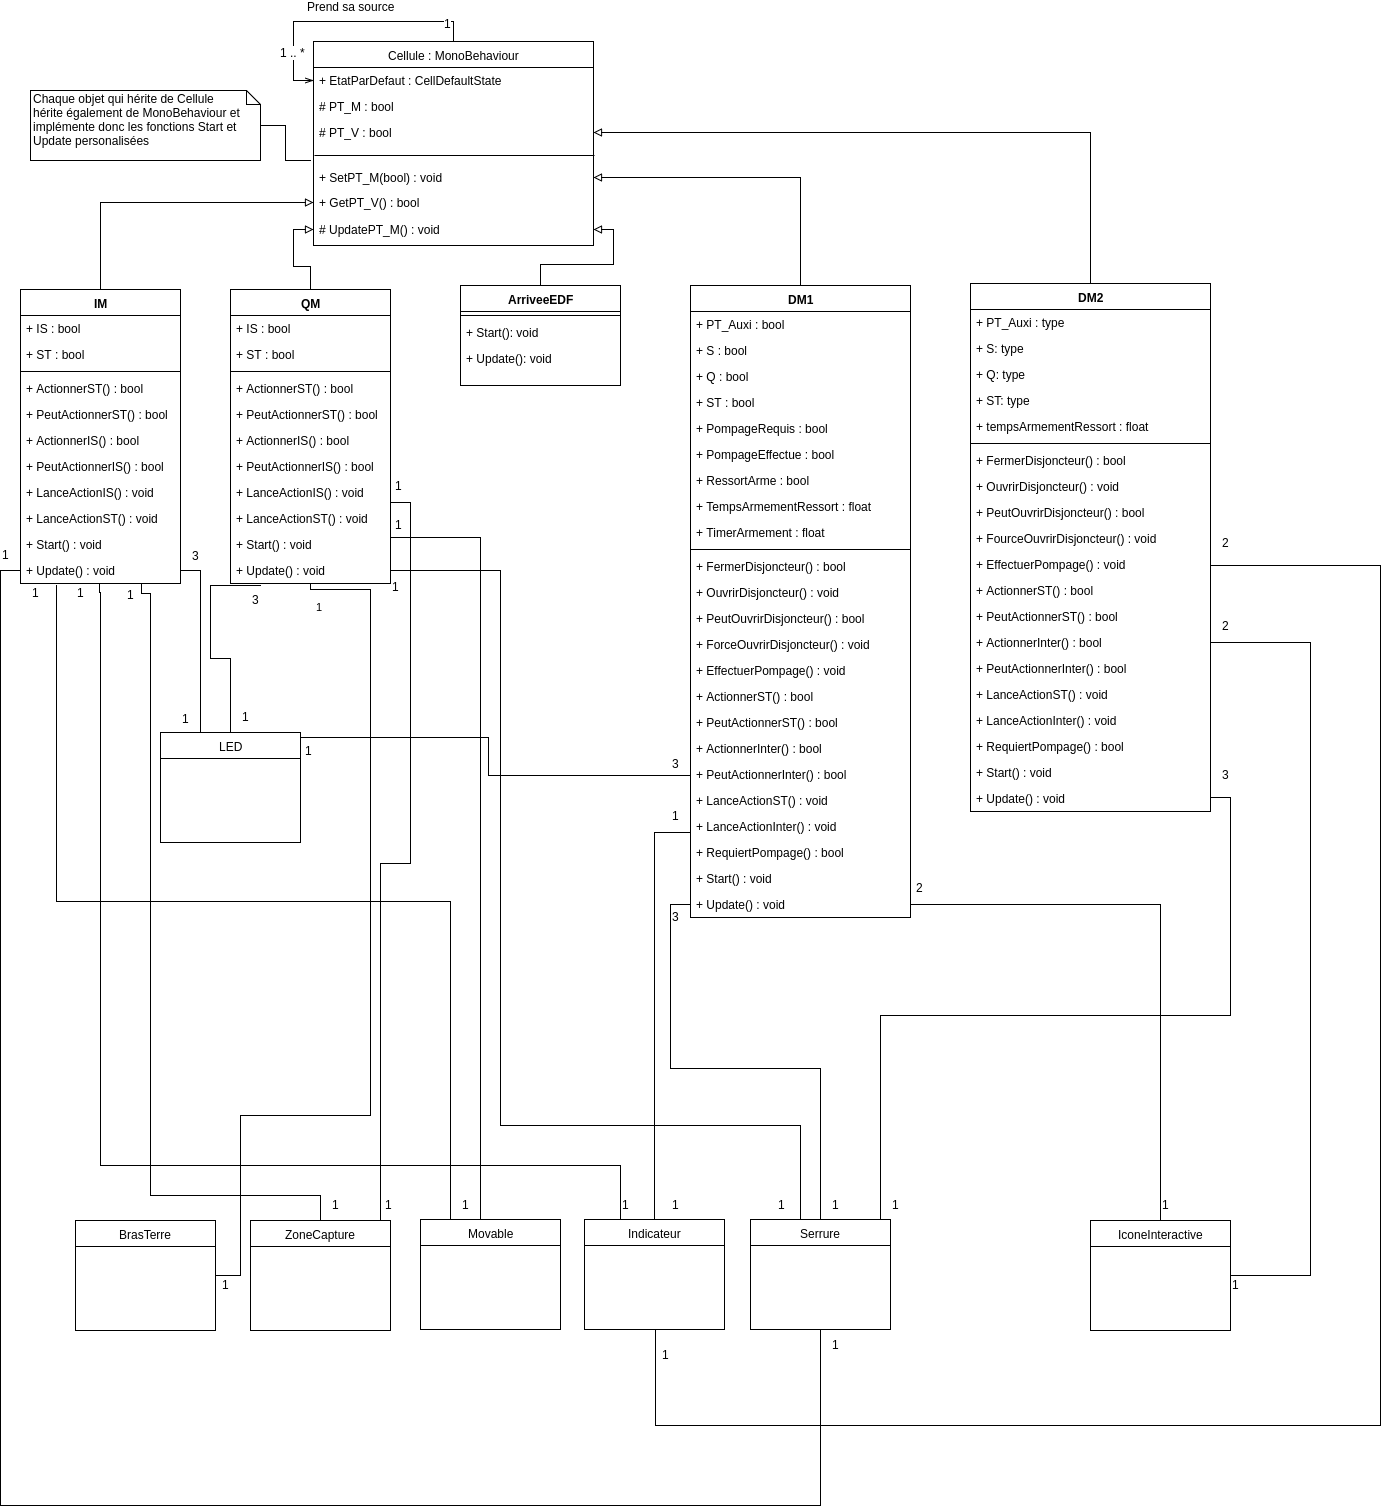
\includegraphics[scale=0.35]{img/DiagClassCellules}
        \caption{Diagramme de classe du système de cellules - Annexe 3}
    \end{figure}

    De plus, j'ai réalisé la simulation du fonctionnement des cellules à haute tension en me basant sur un diagramme d'état-transition, car ces machines sont utilisées en suivant un processus très précis, décrit très simplement par ce diagramme. Voici par exemple celui de la cellule QM \\

    \begin{figure}[H]
        \centering
        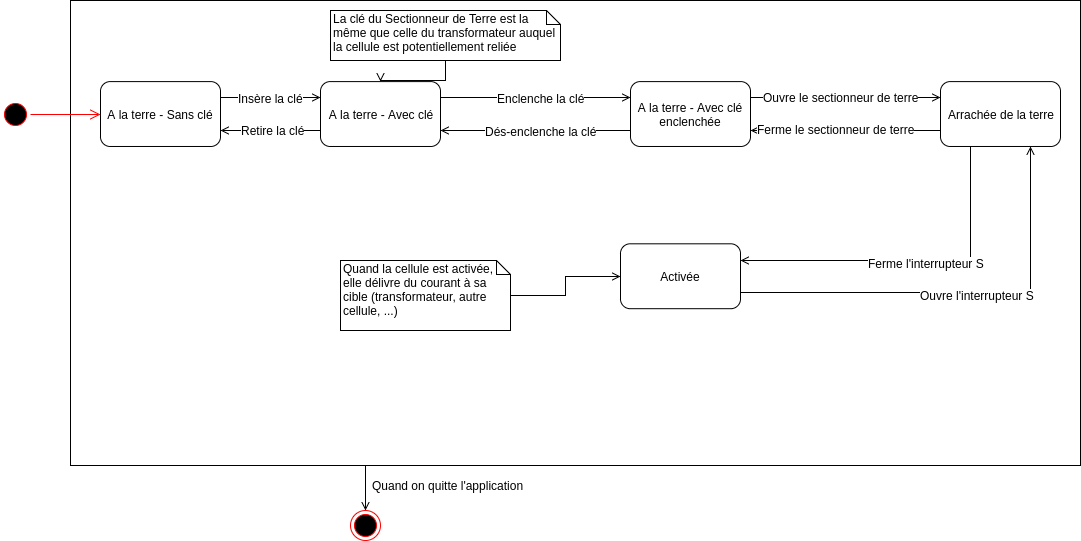
\includegraphics[scale=0.4]{img/DiagEtatTransitionQM}
        \caption{Diagramme d'état-transition représentant le fonctionnement d'une cellule haute tension - Annexe 4}
    \end{figure} 

    \paragraph{Le système de clé / serrures}

    Le système de clé a été une nécéssité rapidement dans le projet. Il permet de bloquer les intéractions possibles avec une cellule si cette dernière n'a pas été sécurisée. Ce système reproduit exactement celui de la réalité. \\

    Les serrures sont identifiées par leur nom, afin de faciliter l'utilisation de ces classes dans les différentes scènes d'Unity. Le système de cellules et de cadenas se basent sur l'utilisation de ces serrures. \\

    Les clés, quant à elles, sont uniquement des objets animés reliés aux serrures. 
    Le fonctionnement a été entièrement expliqué dans la documentation du projet. \\
    
    \begin{figure}[H]
        \centering
        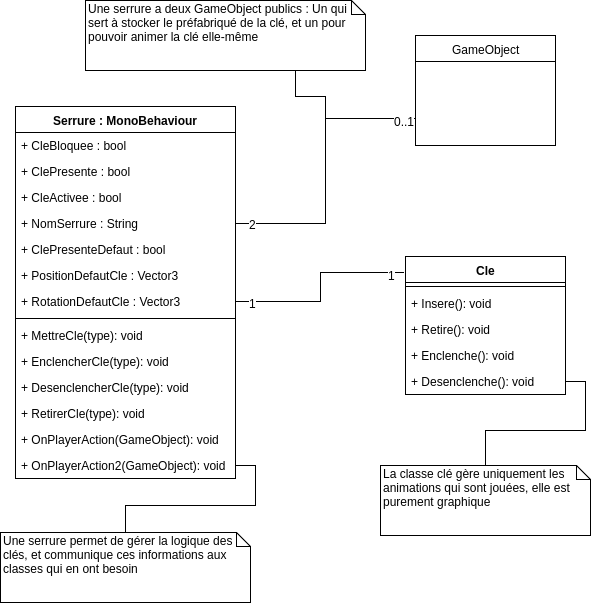
\includegraphics[scale=0.5]{img/DiagClasseSerrures}
        \caption{Diagramme de classe du système de serrures et clés - Annexe 5}
    \end{figure}

    \paragraph{Le système de transformateurs}

    Les transformateurs font partie des derniers objets à avoir été implémenté. Dans la situation réelle, ce sont eux qui se chargent de distribuer le courant issu des cellules haute tension. \\

    Une conception objet a été nécéssaire afin de reproduire le fonctionnement de ces transformateurs. Une fois de plus, le fonctionnement de ces derniers est décrit dans la documentation technique du projet. \\

    \begin{figure}[H]
        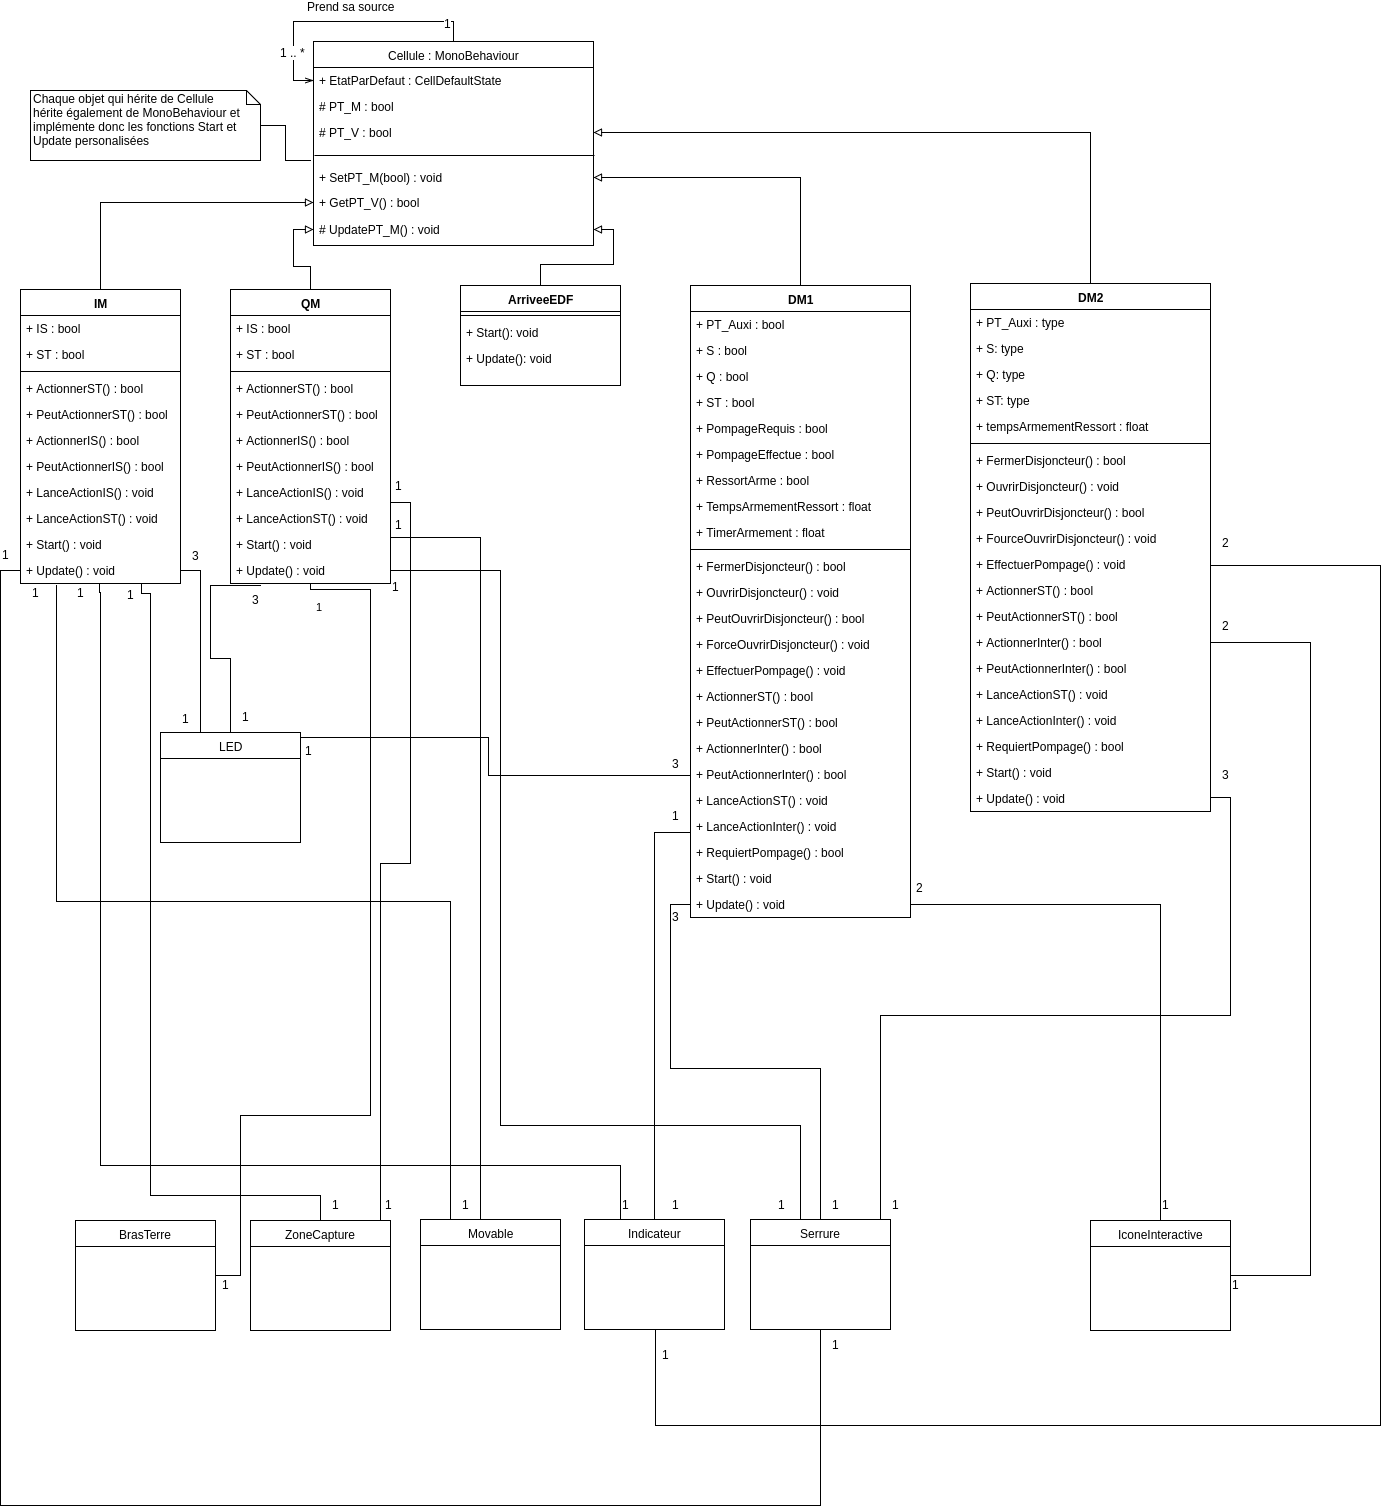
\includegraphics[scale=0.3]{img/DiagClassCellules}
        \caption{Diagramme de classe du système de transformateur - Annexe 6}
    \end{figure}  

    \subsection{Réalisation du projet}

    \subsubsection{Déroulement de la phase de réalisation}
    Beaucoup de retard a été pris sur la réalisation du projet. En effet, la conception n'étant pas possible à effectuer correctement m'a poussé à revenir plusieurs fois sur les mêmes décisions. \\

    La réalisation du projet a été faite suivant une méthode semblable à la méthode Scrum, vue en cours. Chaque jour, je prenais 5 minutes pour discuter avec mon tuteur du travail restant à effectuer, des machines et des interactions qu'il fallait reproduire, et de ce que je pensais réussir à finir dans la journée. Cette sorte de mélée était importante pour garder en tête les objectifs du projet, et me fixer chaque jour un nouveau point à atteindre. \\

    Chaque fois que j'avais un doute, ou besoin d'une information concernant une machine que je ne comprenais pas, ou une interaction à animer, je pouvais contacter mon tuteur de stage par l'intermédiaire de Lync\footnote{Logiciel Microsoft permettant la communication intra-entreprise}. \\

    \begin{figure}[H]
        \centering
        
\includegraphics[scale=0.5]{img/logo-lync}
        \caption{Microsoft Lync}
    \end{figure}

    Chaque partie du projet terminée était soumise à validation par mon tuteur. Il a été décidé également de mettre en place un système de sauvegarde hebdomadaire sur le serveur interne de l'entreprise, permettant de mettre en place un système de versionning\footnote{Se dit d'un système capable de gérer plusieurs versions durant la phase de développement d'un logiciel, permettant le travail à plusieurs collaborateurs et l'accès rapide au code d'une version antérieure} puisque nous n'avons pas utilisé Git ou SVN\footnote{Git et SVN, par exemple, sont deux systèmes de versionning} à cause du manque de serveur interne à l'entreprise. \\

    \begin{figure}[H]
        \centering
        
\includegraphics[scale=0.5]{img/logo-git}
        
\includegraphics[scale=0.15]{img/logo-svn}
        \caption{Git et SVN}
    \end{figure}

    J'ai donc réalisé un script Batch\footnote{Equivalent sous Windows pour les scripts Shell, sorte de petits programmes permettant l'automatisation de tâches systèmes simples} qui a permit d'automatiser la sauvegarde du projet sur le serveur, en respectant les contraintes liées aux projets Unity, c'est à dire en gardant la structure de dossier adéquat. \\

    Vers la moitié du stage, j'ai effectué une démonstration de mon projet auprès de monsieur Renaud Payerne, le chef de projet. Ce dernier a apprécié le rendu graphique, et m'a fait quelques retours sur les attentes qu'il avait par rapport au projet. \\

    \subsubsection{Les difficultés de la réalisation}

    \paragraph{Le système de corde}

    Afin de reproduire le fonctionnement des appareils électriques, il faut également créer le cordon qui relie l'appareil à sa prise. L'utilisation du moteur physique d'Unity pour simuler une corde a été un vrai souci sur lequel j'ai passé une semaine entière de développement. \\

    La solution est triviale à conceptualiser, mais compliquée à mettre en place. En effet, dans un moteur physique, nous pouvons représenter une corde par une suite de corps reliés les uns aux autres par des jointures qui agissent comme des élastiques. \\

    Pour résoudre le problème, j'ai donc crée un script utilisable dans l'éditeur d'Unity qui, une fois l'objet de la corde séléctionné, genère les liaisons physiques adéquates. \\ 

    \begin{figure}[H]
        \centering
        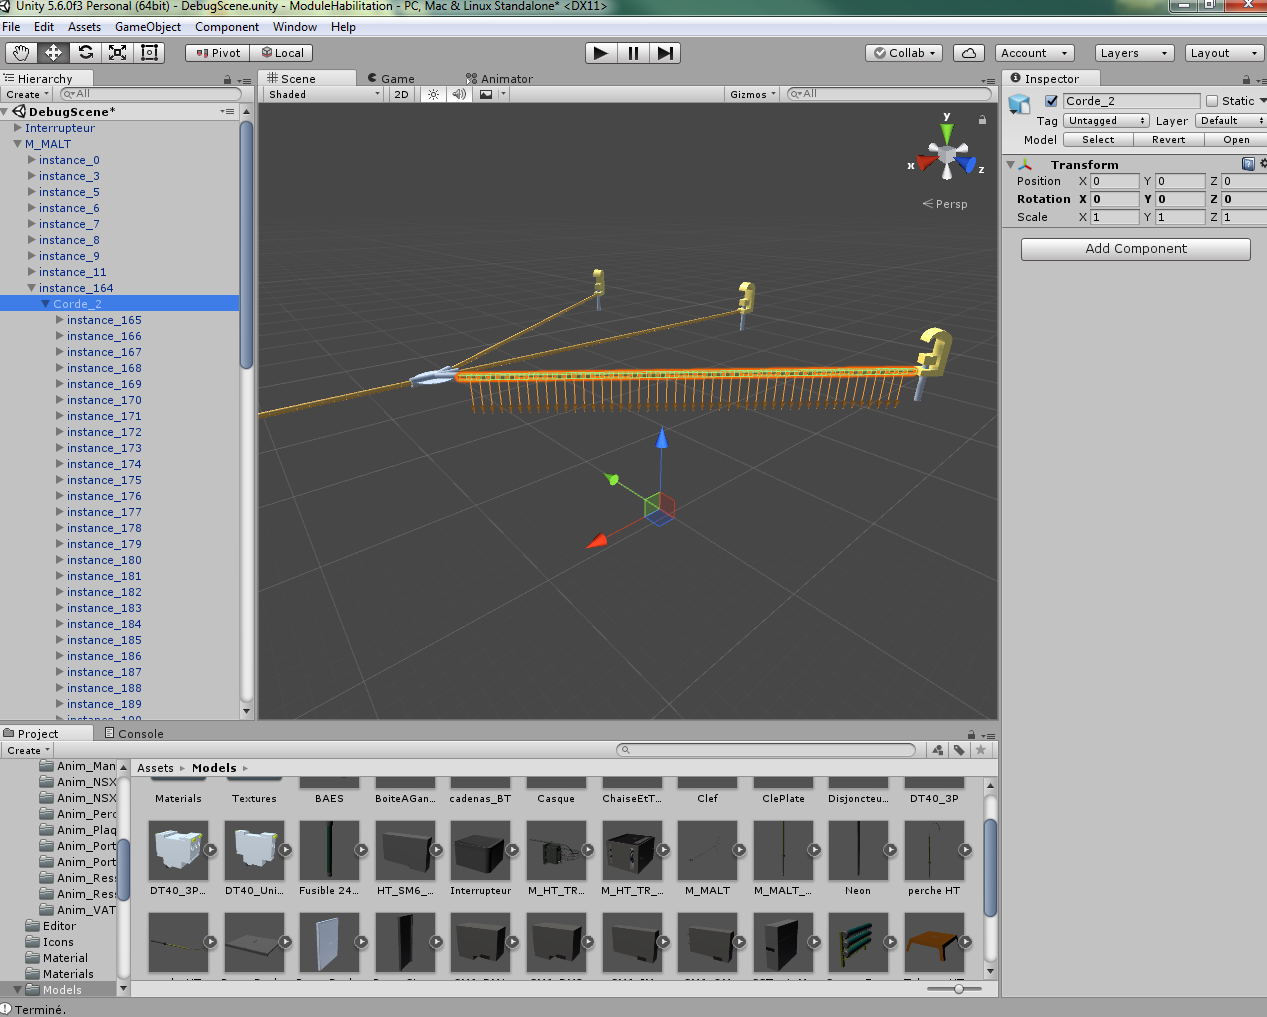
\includegraphics[scale=0.3]{img/CordeUnity}
        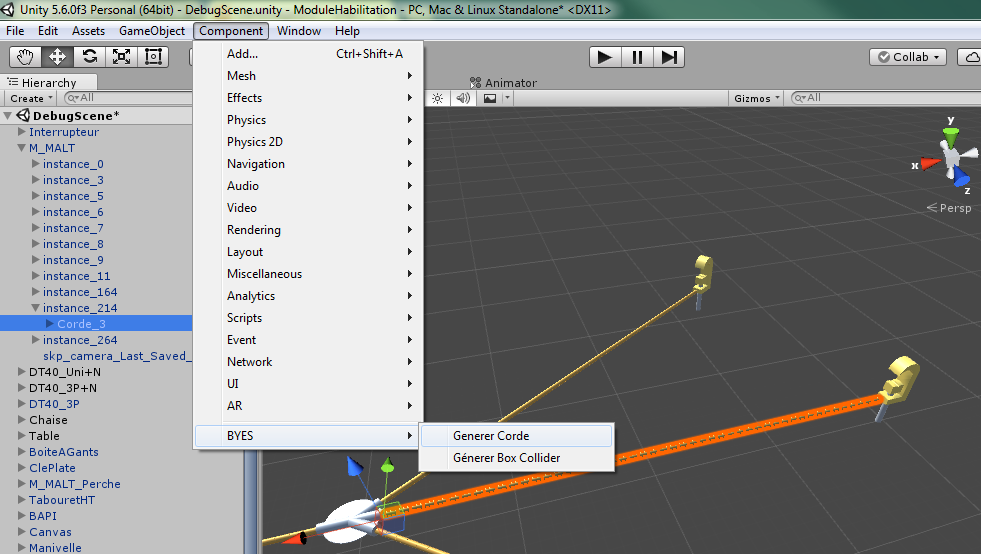
\includegraphics[scale=0.4]{img/GenererCorde}
        \caption{Système de corde dans l'éditeur Unity - Annexe 1}
    \end{figure}

    \paragraph{Les objets portables par l'utilisateur}

    De même, les objets portés par l'utilisateur (comme la clé plate ou la manivelle), ont été un véritable problème à implémenter dans l'application. Ces objets sont soumis au moteur physique d'Unity, afin de garantir le réalisme. \\

    Le problème peut être solutionné de plusieurs façons. J'ai d'abord choisi de me pencher sur la solution d'une jointure physique de type élastique avec un objet invisible, afin de faire en sorte que l'objet suive les déplacements de l'utilsateur dans la simulation. \\

    Déçu par le manque de réalisme de cette solution qui n'avait pas le rendu graphique voulu, j'ai ensuite crée mon propre système afin de pouvoir porter les objets dans le moteur de jeu. Pour résumer le fonctionnement qui est détaillé dans la documentation du projet, on fait en sorte que l'objet bouge tout le temps vers une position cible qui est définie selon l'endroit où l'utilisateur regarde. En annulant les effets du moteur physique sur l'objet, on a ainsi une représentation avec un rendu convenable. \\

    \begin{figure}[H]
        \centering
        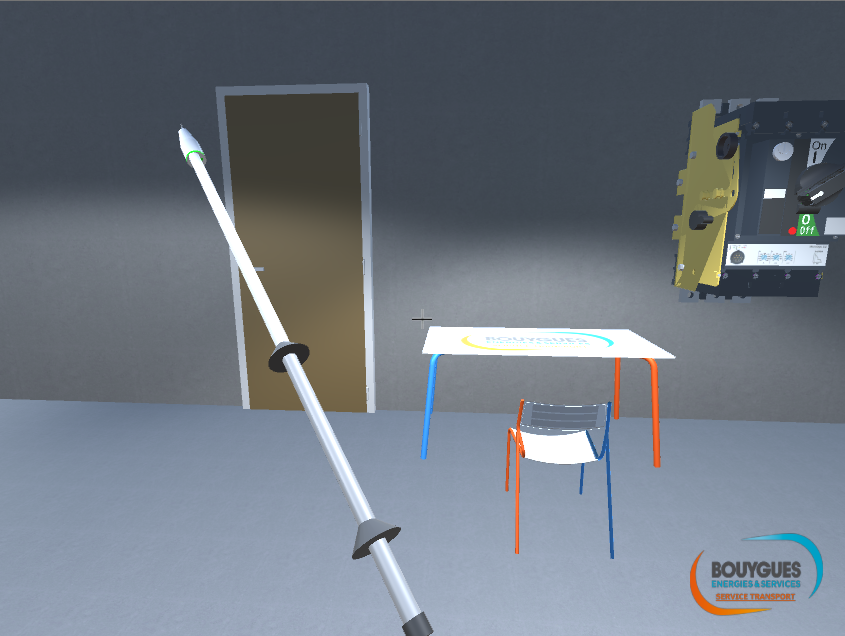
\includegraphics[scale=0.5]{img/SimulPorterObjet}
        \caption{Dans la simulation, l'utilisateur peut porter des objets.}
    \end{figure}

    \subsection{Les tests du projet}

    Unity ne propose pas nativement de système de tests pour les applications qu'il produit. Les tests sont donc effectués à la volée, pendant que je développe. Comme chaque GameObject peut être exporté sous forme de préfabriqué, il suffit pour tester un objet d'importer le préfabriqué et d'étudier son comportement quand on interagit avec.\\

    \subsection{Déploiement de l'application}
   
    Le projet n'a pas été déployé réellement pour l'instant, puisqu'il est toujours en développement et que nous n'avons pas encore réellement implémenté la réalité virtuelle dans l'application, par manque de matériel et de temps. \\

    Il est à noter qu'un système de build\footnote{Export d'une version executable de l'application développée} hebdomadaire a été mis en place : mon tuteur souhaite qu'une version \"utilisable\" de l'application en développement soit toujours à sa disposition. Chaque fin de semaine, en plus de la sauvegarde du projet sur le serveur, j'effectuais donc un export de l'application au format éxecutable. \\
    
    Pour apporter ma contribution à la continuité du développement de l'application, j'ai rédigé une documentation assez précise d'une cinquantaine de pages, en plus d'avoir commenté le code, et d'avoir exporté une documentation en utilisant l'outil Doxygen. \\

    \begin{figure}[H]
        \centering
        
\includegraphics{img/logo-doxygen}
        \caption{Doxygen, outil de documentation pour C\#}
    \end{figure}

    \begin{figure}[H]
        \centering
        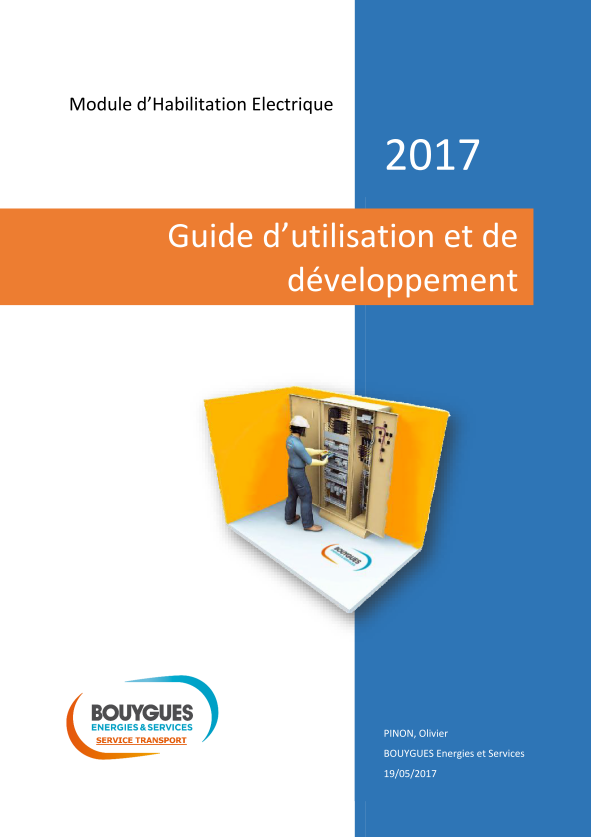
\includegraphics[scale=0.35]{img/DocTechnique1}
        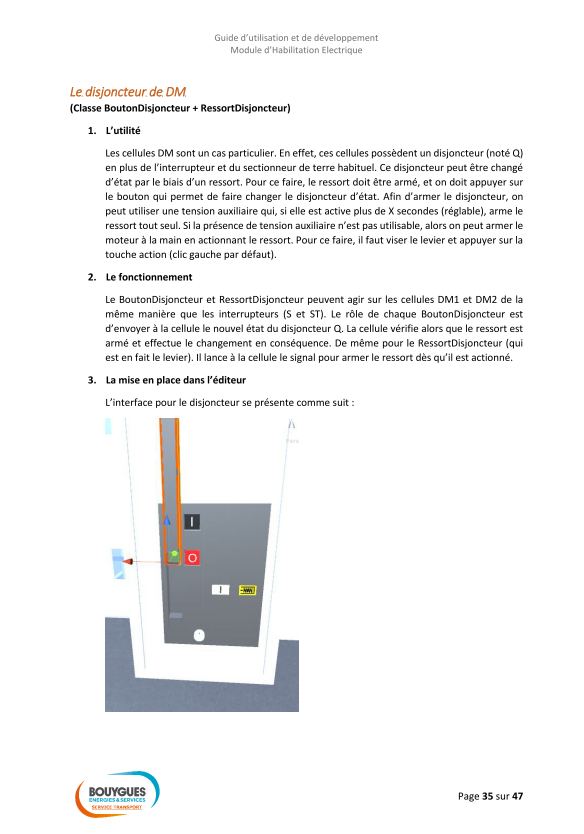
\includegraphics[scale=0.35]{img/DocTechnique2}
        \caption{Captures d'écran de la documentation fournie à l'entreprise}
    \end{figure}

    % Bilan
    \section{Bilan}
    
    \subsection{Bilan personnel}

        Ce stage a été pour moi une véritable source d'enrichissement personnel. Il m'a permit de travailler sur une technologie que j'aime utiliser, dans un cadre de travail très plaisant. \\

        Mes collègues m'ont beaucoup apporté également. Par exemple, un de mes collègues m'a aidé à trouver une alternance pour ma future école d'ingénieur l'année prochaine, en me mettant en relation avec ses contacts. Dans la globalité, le contact avec de nouvelles personnes, des professionnels, a été vraiment un des gros points positifs du stage. \\

        J'ai également eu un aperçu de ce que représente la journée type d'un salarié dans une entreprise. J'ai ainsi compris l'intérêt de la pause du midi, et j'ai eu le confort de pouvoir organiser mes horaires comme je le souhaite, tant que je faisais mes 7 heures quotidiennes. \\

    \subsection{Bilan professionnel}

    Cette experience m'aura également été très bénéfique sur le plan professionnel. En effet, j'ai eu à affronter les difficultés du monde professionnel tout seul, bien que guidé par mon tuteur. J'ai vraiment apprécié cette sensation d'être enfin arrivé au stade où je travaille dans une vraie entreprise, et cela confirme bien mon projet de continuer dans une formation d'ingénieur par apprentissage, afin de rester proche du monde de l'entreprise. \\

    Grâce à ce stage, j'ai également pu apprendre beaucoup de compétences techniques qui vont m'être très utiles dans la suite de mon cursus, notamment dans l'utilisation d'Unity. \\ 

    De plus, j'ai appris énormément sur la communication en entreprise, et les quelques explications techniques que j'ai dû faire auprès de mon tuteur m'ont appris beaucoup sur la vulgarisation qui est nécéssaire pour faire comprendre le développement informatique aux non initiés. \\ 

    J'ai particulièrement apprécié le fait d'avoir un projet concret, et des résultats attendus par des supérieurs hiérarchiques. Ce genre de pression donne envie d'avancer dans le projet. \\
    
    Ce projet concret m'a confronté à la réalité du terrain, et a été un prolongement opérationnel très profitable aux projets d'écoles qui peuvent sembler parfois trop théoriques. Ce stage a donc conclu ma formation de DUT Informatique par une application concrète très appréciable. \\

    % Conclusion
    \huge \textbf{Conclusion} \vspace{5pt} \\
   \normalsize
   
    Ce stage aura été pour moi un vrai succès, autant sur le plan personnel que professionnel. De la montée en compétence à l'intéraction avec mes collèges, la grande majoritée des points sont positifs, et j'ai été très satisfait de mon expérience auprès de Bouygues Energies et Services. \\

    Cette experience m'aura permis de me rendre mieux compte de l'atmosphère de travail dans un grand groupe, et ainsi de valider mon choix d'orientation autour des groupes de plus petite taille, tout du moins dans la suite de ma formation. \\

    La technologie utilisée, le travail que j'ai réalisé, le rythme que j'ai adopté, toutes ces choses ont permis de confirmer mon orientation pour mon projet d'études, mais également mon projet professionnel. Je me suis réellement épanoui dans l'univers où j'ai travaillé, et je souhaite vraiment continuer dans la voie du développement d'applications lourdes, utiliser des moteurs de jeu ou des API graphiques de plus bas niveau. J'ai également découvert mon réel intérêt pour les technologies nouvelles dans l'informatique, comme par exemple la réalité virtuelle. \\

    Le point négatif du stage, la phase de conception qui n'a pas été réalisée correctement, m'aura appris beaucoup sur l'intérêt crucial de la définition du cahier des charges préalable à la mise en oeuvre du projet. J'éprouve également quelques regrets dans le fait de ne pas avoir d'application réellement terminée à ajouter à mon CV. Cette application, qui sera certainement terminée par une autre équipe, est trop incomplète pour être utilisée en production. J'aurais vraiment aimé participer à la phase de déploiement et de maintenance du projet, qui pour moi sont des parties tout aussi importantes que la conception et la réalisation, et qui rendrait mieux compte selon moi du métier d'éditeur de logiciels. \\

    Bien qu'il reste à l'état de protoype, l'objectif de conception d'un module d'habilitation éléctrique est atteint. Ce projet permettra vraisemblabement d'atteindre une nouvelle étape de production d'une future application qui apportera une véritable plus-value à Bouygues Energies et Services. \\

    % Annexes
    \section{Annexes}
    
    \newpage 
    % Page de fin 
    \normalsize
    \thispagestyle{empty}
    \noindent
    \begin{minipage}{.5\textwidth}
        Bouygues Energies et Services \\
        49 avenue du Lac du Bourget \\
        73375 Le Bourget du Lac, France
    \end{minipage}
    \begin{minipage}{.5\textwidth}
    \begin{flushright}
        Pinon Olivier \\
        IUT d'Annecy \\
        DUT INFO \\
        Année 2016/2017 \\
    \end{flushright}
    \end{minipage}

    \vspace{10pt}
    \noindent\rule{0.725\paperwidth}{0.4pt}
    
    \vfill 
    \begin{flushleft}
    \huge \textbf{Résumé : } \\
    \vspace{10pt}
    \normalsize Le secteur de l'industrie s'intéresse de plus en plus aux solutions modernes comme la réalité virtuelle pour répondre à leurs besoins. Afin de créer un nouveau module de formation à l'habilitation éléctrique, j'ai travaillé en collaboration avec le bureau d'études de Bouygues Energies et Services, pour développer une application lourde en réalité virtuelle à l'aide du moteur de jeu Unity et du langage C\#. \\
    \end{flushleft}
    
    \vfill 
    \begin{flushleft}
    \huge \textbf{Mots clefs : } \vspace{2pt} \\
    \vspace{10pt}
    \normalsize Bouygues, Module, Habilitation, Electrique, Réalité, Virtuelle, Unity, 3D, C\#
    \end{flushleft}

    \noindent\rule{0.725\paperwidth}{0.4pt}
    
    \vfill 
    \begin{flushleft}
    \huge \textbf{Abstract : } \\
    \vspace{10pt}
    \normalsize There is a growing interest about virtual reality in the industry sector. In order to fulfil the need of a new electrical habilitation training, I worked in collaboration with the technical studies office of Bouygues Energies and Services, to develop a desktop application in virtual reality using the Unity game engine, and the C\# language.
    \end{flushleft}
    
    \vfill 
    \begin{flushleft}
    \huge \textbf{Keywords : } \\
    \vspace{10pt}
    \normalsize Bouygues, Electrical, Habilitation, Training, Virtual, Reality, Unity, 3D, C\#
    \end{flushleft}

	\vfill
    Palanca Jérôme \hfill Damas Luc
\end{document}
